% Options for packages loaded elsewhere
\PassOptionsToPackage{unicode}{hyperref}
\PassOptionsToPackage{hyphens}{url}
%
\documentclass[
]{article}
\usepackage{amsmath,amssymb}
\usepackage{lmodern}
\usepackage{iftex}
\ifPDFTeX
  \usepackage[T1]{fontenc}
  \usepackage[utf8]{inputenc}
  \usepackage{textcomp} % provide euro and other symbols
\else % if luatex or xetex
  \usepackage{unicode-math}
  \defaultfontfeatures{Scale=MatchLowercase}
  \defaultfontfeatures[\rmfamily]{Ligatures=TeX,Scale=1}
\fi
% Use upquote if available, for straight quotes in verbatim environments
\IfFileExists{upquote.sty}{\usepackage{upquote}}{}
\IfFileExists{microtype.sty}{% use microtype if available
  \usepackage[]{microtype}
  \UseMicrotypeSet[protrusion]{basicmath} % disable protrusion for tt fonts
}{}
\makeatletter
\@ifundefined{KOMAClassName}{% if non-KOMA class
  \IfFileExists{parskip.sty}{%
    \usepackage{parskip}
  }{% else
    \setlength{\parindent}{0pt}
    \setlength{\parskip}{6pt plus 2pt minus 1pt}}
}{% if KOMA class
  \KOMAoptions{parskip=half}}
\makeatother
\usepackage{xcolor}
\IfFileExists{xurl.sty}{\usepackage{xurl}}{} % add URL line breaks if available
\IfFileExists{bookmark.sty}{\usepackage{bookmark}}{\usepackage{hyperref}}
\hypersetup{
  pdftitle={Movielens Movie Recommendation System A Harvard Capstone Project},
  pdfauthor={Manoj Bijoor},
  hidelinks,
  pdfcreator={LaTeX via pandoc}}
\urlstyle{same} % disable monospaced font for URLs
\usepackage[margin=1in]{geometry}
\usepackage{color}
\usepackage{fancyvrb}
\newcommand{\VerbBar}{|}
\newcommand{\VERB}{\Verb[commandchars=\\\{\}]}
\DefineVerbatimEnvironment{Highlighting}{Verbatim}{commandchars=\\\{\}}
% Add ',fontsize=\small' for more characters per line
\newenvironment{Shaded}{}{}
\newcommand{\AlertTok}[1]{\textcolor[rgb]{1.00,0.00,0.00}{\textbf{#1}}}
\newcommand{\AnnotationTok}[1]{\textcolor[rgb]{0.38,0.63,0.69}{\textbf{\textit{#1}}}}
\newcommand{\AttributeTok}[1]{\textcolor[rgb]{0.49,0.56,0.16}{#1}}
\newcommand{\BaseNTok}[1]{\textcolor[rgb]{0.25,0.63,0.44}{#1}}
\newcommand{\BuiltInTok}[1]{#1}
\newcommand{\CharTok}[1]{\textcolor[rgb]{0.25,0.44,0.63}{#1}}
\newcommand{\CommentTok}[1]{\textcolor[rgb]{0.38,0.63,0.69}{\textit{#1}}}
\newcommand{\CommentVarTok}[1]{\textcolor[rgb]{0.38,0.63,0.69}{\textbf{\textit{#1}}}}
\newcommand{\ConstantTok}[1]{\textcolor[rgb]{0.53,0.00,0.00}{#1}}
\newcommand{\ControlFlowTok}[1]{\textcolor[rgb]{0.00,0.44,0.13}{\textbf{#1}}}
\newcommand{\DataTypeTok}[1]{\textcolor[rgb]{0.56,0.13,0.00}{#1}}
\newcommand{\DecValTok}[1]{\textcolor[rgb]{0.25,0.63,0.44}{#1}}
\newcommand{\DocumentationTok}[1]{\textcolor[rgb]{0.73,0.13,0.13}{\textit{#1}}}
\newcommand{\ErrorTok}[1]{\textcolor[rgb]{1.00,0.00,0.00}{\textbf{#1}}}
\newcommand{\ExtensionTok}[1]{#1}
\newcommand{\FloatTok}[1]{\textcolor[rgb]{0.25,0.63,0.44}{#1}}
\newcommand{\FunctionTok}[1]{\textcolor[rgb]{0.02,0.16,0.49}{#1}}
\newcommand{\ImportTok}[1]{#1}
\newcommand{\InformationTok}[1]{\textcolor[rgb]{0.38,0.63,0.69}{\textbf{\textit{#1}}}}
\newcommand{\KeywordTok}[1]{\textcolor[rgb]{0.00,0.44,0.13}{\textbf{#1}}}
\newcommand{\NormalTok}[1]{#1}
\newcommand{\OperatorTok}[1]{\textcolor[rgb]{0.40,0.40,0.40}{#1}}
\newcommand{\OtherTok}[1]{\textcolor[rgb]{0.00,0.44,0.13}{#1}}
\newcommand{\PreprocessorTok}[1]{\textcolor[rgb]{0.74,0.48,0.00}{#1}}
\newcommand{\RegionMarkerTok}[1]{#1}
\newcommand{\SpecialCharTok}[1]{\textcolor[rgb]{0.25,0.44,0.63}{#1}}
\newcommand{\SpecialStringTok}[1]{\textcolor[rgb]{0.73,0.40,0.53}{#1}}
\newcommand{\StringTok}[1]{\textcolor[rgb]{0.25,0.44,0.63}{#1}}
\newcommand{\VariableTok}[1]{\textcolor[rgb]{0.10,0.09,0.49}{#1}}
\newcommand{\VerbatimStringTok}[1]{\textcolor[rgb]{0.25,0.44,0.63}{#1}}
\newcommand{\WarningTok}[1]{\textcolor[rgb]{0.38,0.63,0.69}{\textbf{\textit{#1}}}}
\usepackage{graphicx}
\makeatletter
\def\maxwidth{\ifdim\Gin@nat@width>\linewidth\linewidth\else\Gin@nat@width\fi}
\def\maxheight{\ifdim\Gin@nat@height>\textheight\textheight\else\Gin@nat@height\fi}
\makeatother
% Scale images if necessary, so that they will not overflow the page
% margins by default, and it is still possible to overwrite the defaults
% using explicit options in \includegraphics[width, height, ...]{}
\setkeys{Gin}{width=\maxwidth,height=\maxheight,keepaspectratio}
% Set default figure placement to htbp
\makeatletter
\def\fps@figure{htbp}
\makeatother
% Make links footnotes instead of hotlinks:
\DeclareRobustCommand{\href}[2]{#2\footnote{\url{#1}}}
\setlength{\emergencystretch}{3em} % prevent overfull lines
\providecommand{\tightlist}{%
  \setlength{\itemsep}{0pt}\setlength{\parskip}{0pt}}
\setcounter{secnumdepth}{5}
\usepackage[utf8]{inputenc} \usepackage[english]{babel} \usepackage[]{hyperref} \hypersetup{ backref, colorlinks=true, linkcolor=blue, filecolor=magenta, urlcolor=cyan, pdftitle={"Movielens Harvard Capstone"}, bookmarks=true, pdfpagemode=FullScreen, pdfstartpage=1, hyperindex=true, pageanchor=true, } \usepackage{amsmath} \usepackage{pdflscape} \usepackage[titles]{tocloft} \usepackage{tocloft} \usepackage{titlesec} \usepackage{longtable} \usepackage{xpatch} \usepackage[T1]{fontenc} \usepackage{imakeidx} \makeindex[columns=3, title=Alphabetical Index, intoc]
\usepackage{subfig}
\usepackage{booktabs}
\usepackage{longtable}
\usepackage{array}
\usepackage{multirow}
\usepackage{wrapfig}
\usepackage{float}
\usepackage{colortbl}
\usepackage{pdflscape}
\usepackage{tabu}
\usepackage{threeparttable}
\usepackage{threeparttablex}
\usepackage[normalem]{ulem}
\usepackage{makecell}
\usepackage{xcolor}
\ifLuaTeX
  \usepackage{selnolig}  % disable illegal ligatures
\fi

\title{Movielens\\
Movie Recommendation System\\
A Harvard Capstone Project}
\author{Manoj Bijoor}
\date{March 14, 2021}

\begin{document}
\maketitle

\pagenumbering{roman}

\newpage

\newpage

\begin{center}

\large{Abstract}

\end{center}

\bigskip

\ldots this is the abstract text\ldots{}

\newpage 
\clearpage
\phantomsection
\setcounter{secnumdepth}{5}
\setcounter{tocdepth}{5}

\tableofcontents
\clearpage

\newpage
\clearpage
\phantomsection

\hypertarget{list-of-tables}{%
\section*{List of tables}\label{list-of-tables}}
\addcontentsline{toc}{section}{List of tables}

\renewcommand{\listtablename}{}

\listoftables
\clearpage

\newpage
\clearpage
\phantomsection

\hypertarget{list-of-figures}{%
\section*{List of figures}\label{list-of-figures}}
\addcontentsline{toc}{section}{List of figures}

\renewcommand{\listfigurename}{}

\listoffigures
\clearpage

\newpage
\clearpage
\phantomsection
\newcommand{\listequationsname}{List of Equations}
\newlistof{equations}{equ}{List of Equations}
\newcommand{\equations}[1]{%
\refstepcounter{equations}
\par\noindent\textbf{equations \theequations. #1}
\addcontentsline{equ}{equations}{\thesection. \protect\numberline{\theequations}#1}\par}
\xpretocmd{\listofequations}{\addcontentsline{toc}{section}{List of Equations}}{}{}

\makeatletter
\let\l@equations\l@figure
\makeatother

\renewcommand{\listequationsname}{}

\listofequations
\clearpage

\newpage

\pagenumbering{arabic}

\hypertarget{project-overview-movielens---a-harvard-capstone-project}{%
\section{Project Overview: MovieLens - A Harvard Capstone
Project}\label{project-overview-movielens---a-harvard-capstone-project}}

A movie recommendation system using the MovieLens dataset.

For this project, I will be creating a movie recommendation system using
the MovieLens dataset, provided by
\href{https://grouplens.org/}{GroupLens Research}, a research lab in the
Department of Computer Science and Engineering at the University of
Minnesota, Twin Cities specializing in recommender systems, online
communities, mobile and ubiquitous technologies, digital libraries, and
local geographic information systems.

\href{https://grouplens.org/datasets/movielens/}{GroupLens Research} has
collected and made available rating data sets from the
\href{https://movielens.org}{MovieLens web site}. The data sets were
collected over various periods of time, depending on the size of the
set.

I will use the \href{https://grouplens.org/datasets/movielens/10m/}{10M
version of the MovieLens dataset} to make the computation a little
easier.

\textbf{First}, I will download the MovieLens data and run code provided
to generate my datasets.

\textbf{Second}, I will train a machine learning algorithm using the
inputs in one subset to predict movie ratings in the validation set.

\hypertarget{create-train-and-final-hold-out-test-sets}{%
\subsection{Create Train and Final Hold-out Test
Sets}\label{create-train-and-final-hold-out-test-sets}}

I will develop my algorithm using the edx set. For a final test of my
final algorithm, I predict movie ratings in the validation set (the
final hold-out test set) as if they were unknown.
\href{https://en.wikipedia.org/wiki/Root-mean-square_deviation}{RMSE}
will be used to evaluate how close my predictions are to the true values
in the validation set (the final hold-out test set).

\hypertarget{important-data-sets-usage}{%
\subsubsection{Important: Data sets
usage}\label{important-data-sets-usage}}

The validation data (the final hold-out test set) will NOT be used for
training, developing, or selecting my algorithm and it will ONLY be used
for evaluating the RMSE of my final algorithm. The final hold-out test
set will only be used at the end of my project with my final model. It
will not be used to test the RMSE of multiple models during model
development. I will split the edx data into separate training and test
sets to design and test my algorithm.

\hypertarget{final-product}{%
\subsection{Final Product}\label{final-product}}

\hypertarget{my-submission-for-this-project-is-three-files}{%
\subsubsection{My submission for this project is three
files:}\label{my-submission-for-this-project-is-three-files}}

\begin{enumerate}
\def\labelenumi{\arabic{enumi}.}
\tightlist
\item
  My report in Rmd format
\item
  My report in PDF format (knit from my Rmd file)
\item
  A script in R format that generates my predicted movie ratings and
  RMSE score (contains all code and comments for my project)
\end{enumerate}

The report documents the analysis and presents the findings, along with
supporting statistics and figures. The report assumes that the reader is
not familiar with the project or the data. The report includes the RMSE
generated and the following sections:\\
1. an introduction/overview/executive summary section that describes the
dataset and summarizes the goal of the project and key steps that were
performed 2. a methods/analysis section that explains the process and
techniques used, including data cleaning, data exploration and
visualization, insights gained, and my modeling approach 3. a results
section that presents the modeling results and discusses the model
performance 4. a conclusion section that gives a brief summary of the
report, its limitations and future work

\newpage

\hypertarget{exploratory-data-analysis}{%
\section{Exploratory Data Analysis}\label{exploratory-data-analysis}}

\hypertarget{data-wrangling}{%
\subsection{Data Wrangling}\label{data-wrangling}}

\href{https://en.wikipedia.org/wiki/Data_wrangling}{Data wrangling},
sometimes referred to as data munging, is the process of transforming
and mapping data from one ``raw'' data form into another format with the
intent of making it more appropriate and valuable for a variety of
downstream purposes such as analytics.

The main steps could be described as follows:\\
1. Discovering\\
2. Structuring\\
3. Cleaning\\
4. Enriching\\
5. Validating\\
6. Publishing

Let's perform the steps or combinations thereof starting with Initial
data Exploration \& Visualization in the next few subsections.

\hypertarget{initial-data-exploration-visualization}{%
\subsubsection{Initial data Exploration \&
Visualization}\label{initial-data-exploration-visualization}}

The first ten rows out of 9000055 rows of the Movielens data can be
found in Table \ref{tbl:movielens_data}.

\begin{table}[H]

\caption{\label{tab:eda_1}Movielens data\label{tbl:movielens_data}}
\centering
\fontsize{7}{9}\selectfont
\begin{tabular}[t]{rrrrll}
\toprule
userId & movieId & rating & timestamp & title & genres\\
\midrule
1 & 122 & 5 & 838985046 & Boomerang (1992) & Comedy|Romance\\
1 & 185 & 5 & 838983525 & Net, The (1995) & Action|Crime|Thriller\\
1 & 292 & 5 & 838983421 & Outbreak (1995) & Action|Drama|Sci-Fi|Thriller\\
1 & 316 & 5 & 838983392 & Stargate (1994) & Action|Adventure|Sci-Fi\\
1 & 329 & 5 & 838983392 & Star Trek: Generations (1994) & Action|Adventure|Drama|Sci-Fi\\
1 & 355 & 5 & 838984474 & Flintstones, The (1994) & Children|Comedy|Fantasy\\
1 & 356 & 5 & 838983653 & Forrest Gump (1994) & Comedy|Drama|Romance|War\\
1 & 362 & 5 & 838984885 & Jungle Book, The (1994) & Adventure|Children|Romance\\
1 & 364 & 5 & 838983707 & Lion King, The (1994) & Adventure|Animation|Children|Drama|Musical\\
1 & 370 & 5 & 838984596 & Naked Gun 33 1/3: The Final Insult (1994) & Action|Comedy\\
\bottomrule
\end{tabular}
\end{table}

Each row represents a rating given by one user to one movie.

We can see the number of unique users that provided ratings and how many
unique movies were rated. The unique genres here is based on a column
called ``genres'' that includes every genre that applies to the movie.
Some movies fall under several genres. Defining a category as whatever
combination appears in this column, we are going to refer to this
category as ``unique genres'' or simply ``genres'' from now on.

The number of unique users, movies and genres can be found in Table
\ref{tbl:uniq_users_movies_genres}.

\begin{table}[H]

\caption{\label{tab:eda_2}Unique Users, Movies and Genres\label{tbl:uniq_users_movies_genres}}
\centering
\begin{tabular}[t]{rrr}
\toprule
unique\_users & unique\_movies & unique\_genres\\
\midrule
69878 & 10677 & 797\\
\bottomrule
\end{tabular}
\end{table}

If we multiply the number of unique users by number of unique movies, we
get a very large number, actually 746087406, yet our data table has
9000055 rows. This implies that not every user rated every movie. So we
can think of these data as a very large matrix, with users on the rows
and movies on the columns, with many empty cells. The `gather' function
permits us to convert it to this format, but if we try it for the entire
matrix, it will crash R.

Let's show the matrix of seven users ie: userId's 13-20 and four movies
in Table \ref{tbl:matrix_seven_users_four_movies}.

\begin{table}[H]

\caption{\label{tab:eda_3}Matrix of seven users and four movies\label{tbl:matrix_seven_users_four_movies}}
\centering
\fontsize{8}{10}\selectfont
\begin{tabular}[t]{rrrrr}
\toprule
userId & Forrest Gump (1994) & Jurassic Park (1993) & Pulp Fiction (1994) & Silence of the Lambs, The (1991)\\
\midrule
13 & NA & NA & 4 & NA\\
16 & NA & 3 & NA & NA\\
17 & NA & NA & NA & 5\\
18 & NA & 3 & 5 & 5\\
19 & 4 & 1 & NA & NA\\
\bottomrule
\end{tabular}
\end{table}

\newpage

\hypertarget{a-very-sparse-matrix}{%
\paragraph{A Very Sparse Matrix}\label{a-very-sparse-matrix}}

You can think of the task of a recommendation system as filling in the
`NAs' in the table above. To see how sparse the matrix is, here is the
matrix in Figure \ref{fig:matr} for a random sample of 100 movies and
100 users with yellow indicating a user/movie combination for which we
have a rating.

\begin{figure}
\centering
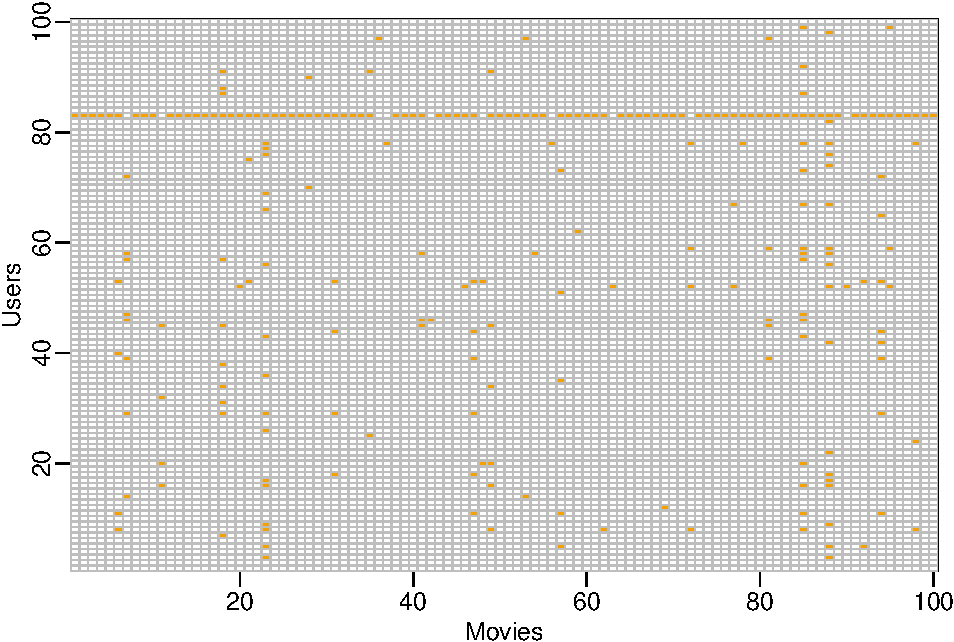
\includegraphics{figures/eda_4-1.pdf}
\caption{A Very Sparse Matrix\label{fig:matr}}
\end{figure}

This machine learning challenge is quite complicated, because each
outcome \(Y\) has a different set of predictors. To see this, note that
if we are predicting the rating for movie \emph{i} by user \emph{u}, in
principle, all other ratings related to movie \emph{i} and by user
\emph{u} may be used as predictors, but different users rate different
movies and a different number of movies. Furthermore, we may be able to
use information from other movies that we have determined are similar to
movie \emph{i} or from users determined to be similar to user \emph{u}.
In essence, the entire matrix can be used as predictors for each cell.

\newpage

\hypertarget{general-properties-of-the-data}{%
\paragraph{General Properties of the
data}\label{general-properties-of-the-data}}

Let's look at some of the \textbf{\emph{general properties}} of the data
to better understand the challenges.

The \textbf{\emph{first thing}} we notice is that some movies get rated
more than others. Figure \ref{fig:movies_getting_rated} shows the Movies
getting rated distribution. This should not surprise us given that there
are blockbuster movies watched by millions and artsy, independent movies
watched by just a few:

\begin{figure}
\centering
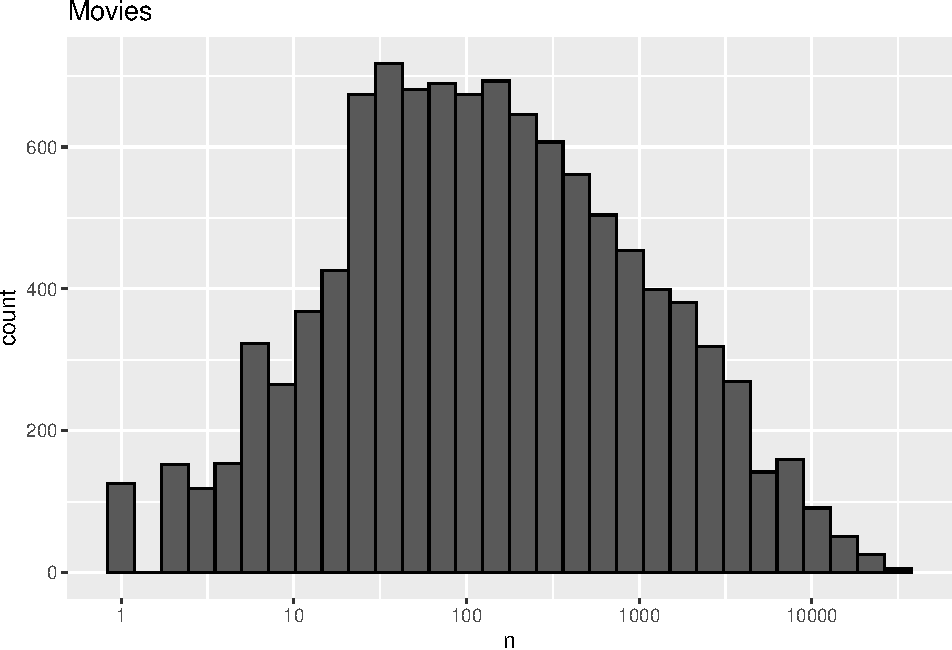
\includegraphics{figures/eda_5-1.pdf}
\caption{Movies getting rated
distribution\label{fig:movies_getting_rated}}
\end{figure}

\newpage

Our \textbf{\emph{second observation}} is that some users are more
active than others at rating movies. Figure
\ref{fig:users_rating_movies} shows Users rating movies distribution:

\begin{figure}
\centering
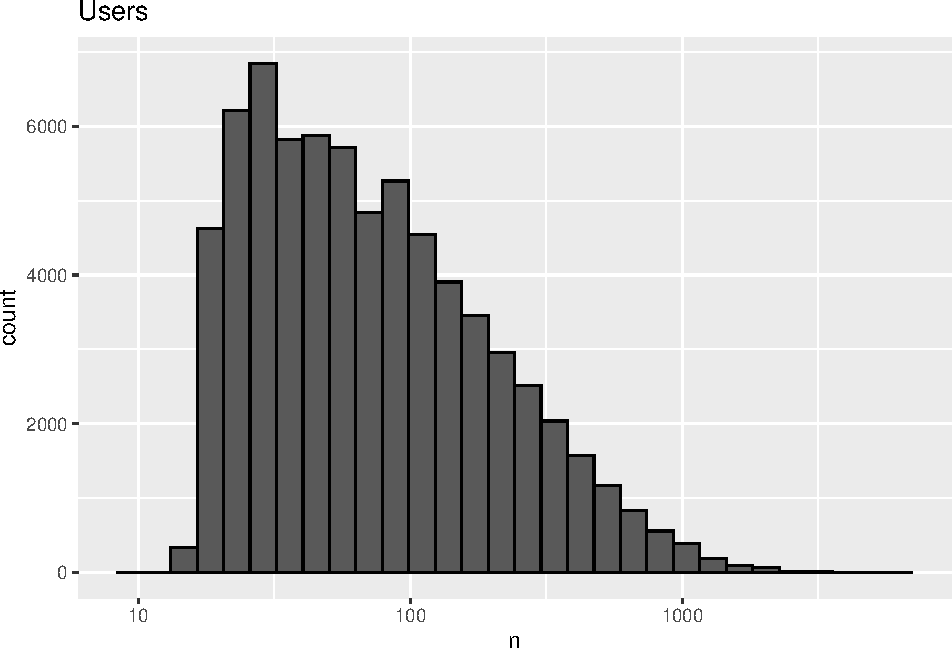
\includegraphics{figures/eda_6-1.pdf}
\caption{Users rating movies
distribution\label{fig:users_rating_movies}}
\end{figure}

\newpage

\hypertarget{further-data-exploration-visualization-modification}{%
\subsubsection{Further data Exploration, Visualization \&
Modification}\label{further-data-exploration-visualization-modification}}

\hypertarget{modify_edx}{%
\paragraph{Modify edx}\label{modify_edx}}

\textbf{Convert timestamp} in Movielens edx data Table
\ref{tbl:movielens_data} into date-time, a more readable and useful
format named \emph{rating\_date} in Table
\ref{tbl:movielens_edx_data_rating_date} below.

\begin{table}[H]

\caption{\label{tab:dw_1}Movielens edx data with rating date-time\label{tbl:movielens_edx_data_rating_date}}
\centering
\fontsize{8}{10}\selectfont
\begin{tabular}[t]{rrrlll}
\toprule
userId & movieId & rating & title & genres & rating\_date\\
\midrule
1 & 122 & 5 & Boomerang (1992) & Comedy|Romance & 1996-08-02 11:24:06\\
1 & 185 & 5 & Net, The (1995) & Action|Crime|Thriller & 1996-08-02 10:58:45\\
1 & 292 & 5 & Outbreak (1995) & Action|Drama|Sci-Fi|Thriller & 1996-08-02 10:57:01\\
1 & 316 & 5 & Stargate (1994) & Action|Adventure|Sci-Fi & 1996-08-02 10:56:32\\
1 & 329 & 5 & Star Trek: Generations (1994) & Action|Adventure|Drama|Sci-Fi & 1996-08-02 10:56:32\\
\bottomrule
\end{tabular}
\end{table}

\textbf{Split title} in Movielens edx data Table
\ref{tbl:movielens_data} into title and year movie released, a more
useful format named \emph{movie\_dt} in Table
\ref{tbl:movielens_edx_movie_release_date} below.

\begin{table}[H]

\caption{\label{tab:dw_2}Movielens edx data with movie release date\label{tbl:movielens_edx_movie_release_date}}
\centering
\fontsize{8}{10}\selectfont
\begin{tabular}[t]{rrrlllr}
\toprule
userId & movieId & rating & title & genres & rating\_date & movie\_dt\\
\midrule
1 & 122 & 5 & Boomerang & Comedy|Romance & 1996-08-02 11:24:06 & 1992\\
1 & 185 & 5 & Net, The & Action|Crime|Thriller & 1996-08-02 10:58:45 & 1995\\
1 & 292 & 5 & Outbreak & Action|Drama|Sci-Fi|Thriller & 1996-08-02 10:57:01 & 1995\\
1 & 316 & 5 & Stargate & Action|Adventure|Sci-Fi & 1996-08-02 10:56:32 & 1994\\
1 & 329 & 5 & Star Trek: Generations & Action|Adventure|Drama|Sci-Fi & 1996-08-02 10:56:32 & 1994\\
\bottomrule
\end{tabular}
\end{table}

\newpage

\hypertarget{modify-validation-repeat-above-steps}{%
\paragraph{Modify validation, repeat above
steps}\label{modify-validation-repeat-above-steps}}

\textbf{Convert timestamp} in Movielens validation data Table
\ref{tbl:movielens_data} into date-time, a more readable and useful
format named \emph{rating\_date} in Table
\ref{tbl:movielens_val_data_rating_date} below.

\begin{table}[H]

\caption{\label{tab:dw_3}Movielens validation data with rating date-time\label{tbl:movielens_val_data_rating_date}}
\centering
\fontsize{8}{10}\selectfont
\begin{tabular}[t]{rrrlll}
\toprule
userId & movieId & rating & title & genres & rating\_date\\
\midrule
1 & 231 & 5 & Dumb \& Dumber (1994) & Comedy & 1996-08-02 10:56:32\\
1 & 480 & 5 & Jurassic Park (1993) & Action|Adventure|Sci-Fi|Thriller & 1996-08-02 11:00:53\\
1 & 586 & 5 & Home Alone (1990) & Children|Comedy & 1996-08-02 11:07:48\\
2 & 151 & 3 & Rob Roy (1995) & Action|Drama|Romance|War & 1997-07-07 03:34:10\\
2 & 858 & 2 & Godfather, The (1972) & Crime|Drama & 1997-07-07 03:20:45\\
\bottomrule
\end{tabular}
\end{table}

\textbf{Split title} in Movielens validation data Table
\ref{tbl:movielens_data} into title and year movie released, a more
useful format named \emph{movie\_dt} in Table
\ref{tbl:movielens_val_movie_release_date} below.

\begin{table}[H]

\caption{\label{tab:dw_4}Movielens validation data with movie release date\label{tbl:movielens_val_movie_release_date}}
\centering
\fontsize{8}{10}\selectfont
\begin{tabular}[t]{rrrlllr}
\toprule
userId & movieId & rating & title & genres & rating\_date & movie\_dt\\
\midrule
1 & 231 & 5 & Dumb \& Dumber & Comedy & 1996-08-02 10:56:32 & 1994\\
1 & 480 & 5 & Jurassic Park & Action|Adventure|Sci-Fi|Thriller & 1996-08-02 11:00:53 & 1993\\
1 & 586 & 5 & Home Alone & Children|Comedy & 1996-08-02 11:07:48 & 1990\\
2 & 151 & 3 & Rob Roy & Action|Drama|Romance|War & 1997-07-07 03:34:10 & 1995\\
2 & 858 & 2 & Godfather, The & Crime|Drama & 1997-07-07 03:20:45 & 1972\\
\bottomrule
\end{tabular}
\end{table}

\newpage

\hypertarget{movie-release-date---a-closer-look}{%
\paragraph{Movie Release Date - a closer
look}\label{movie-release-date---a-closer-look}}

Computing the number of ratings for each movie and then plotting it
against the year the movie came out, that is the release date and using
the square root transformation on the counts using Table
\ref{tbl:movielens_edx_movie_release_date} , we get see Figure
\ref{fig:ratings_movie_release_date_all_dates} :

\begin{figure}[h!]

{\centering \subfloat[All data points only\label{fig:md_1-1}]{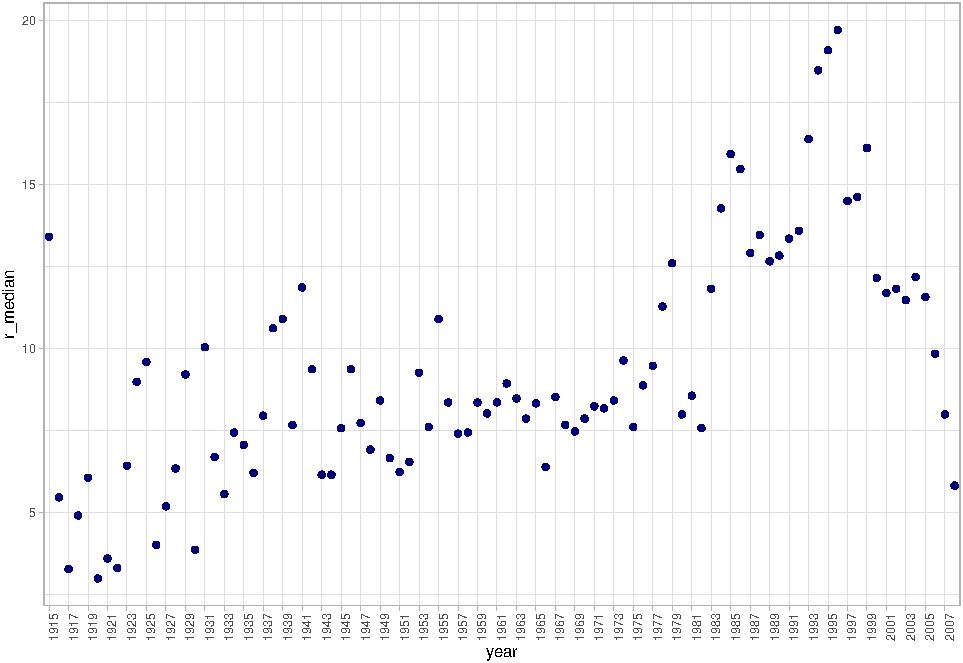
\includegraphics[width=0.7\linewidth]{figures/md_1-1} }\newline\subfloat[Smooth line through all data points\label{fig:md_1-2}]{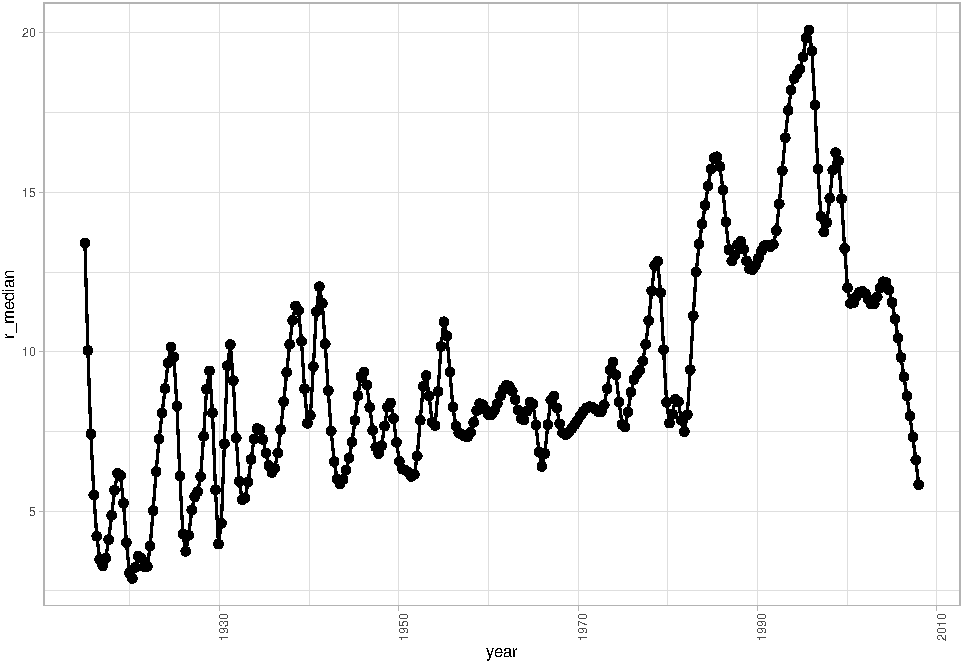
\includegraphics[width=0.7\linewidth]{figures/md_1-2} }

}

\caption{Ratings Movie Release Date - All dates\label{fig:ratings_movie_release_date_all_dates}}\label{fig:md_1}
\end{figure}

we see that, on average, movies that came out after 1993 get more
ratings. We also see that with newer movies, starting in 1993, the
number of ratings decreases with year: the more recent a movie is, the
less time users have had to rate it.

\newpage

Among movies that came out in 1991 or later, we select the top 25 movies
with the highest average number of ratings per year (n/year) and
calculate the average rating of each of them. To calculate number of
ratings per year, use 2018 as the end year. See Figure
\ref{fig:25_movies_avg_and_most_ratings_per_year_post_1991} :

\begin{verbatim}
`geom_smooth()` using method = 'loess' and formula 'y ~ x'
\end{verbatim}

\begin{figure}
\centering
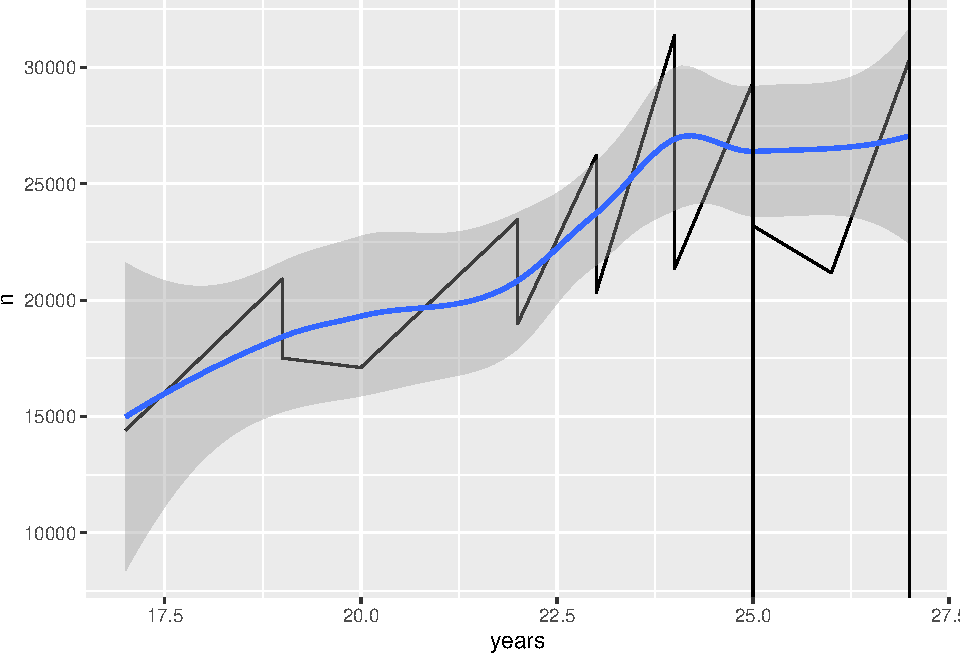
\includegraphics{figures/md_2-1.pdf}
\caption{25 Movies with the most ratings per year and their average
rating post
1991\label{fig:25_movies_avg_and_most_ratings_per_year_post_1991}}
\end{figure}

\newpage

Among movies that came out in 1993 or later, we select the top 25 movies
with the highest average number of ratings per year (n/year) and
calculate the average rating of each of them. To calculate number of
ratings per year, use 2018 as the end year. See Figure
\ref{fig:25_movies_avg_and_most_ratings_per_year_post_1993} :

\begin{verbatim}
`geom_smooth()` using method = 'loess' and formula 'y ~ x'
\end{verbatim}

\begin{figure}
\centering
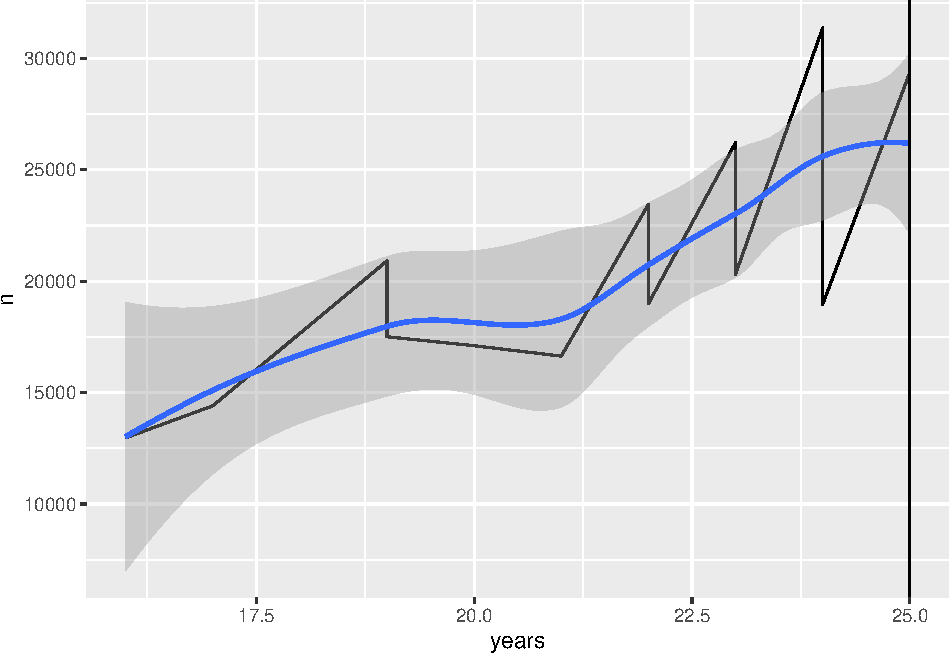
\includegraphics{figures/md_3-1.pdf}
\caption{25 Movies with the most ratings per year and their average
rating post
1993\label{fig:25_movies_avg_and_most_ratings_per_year_post_1993}}
\end{figure}

\newpage

We see that the most rated movies tend to have above average ratings.
This is not surprising: more people watch popular movies. To confirm
this, we stratify the post 1993 movies by ratings per year and compute
their average ratings. Figure
\ref{fig:movies_average_ratings_versus_ratings_per_year_post_1993} is a
plot of average ratings versus ratings per year showing an estimate of
the trend.

We see that the more a movie is rated, the higher the rating.

\textbf{Post-1993 movies}

\begin{verbatim}
`geom_smooth()` using method = 'gam' and formula 'y ~ s(x, bs = "cs")'
\end{verbatim}

\begin{figure}
\centering
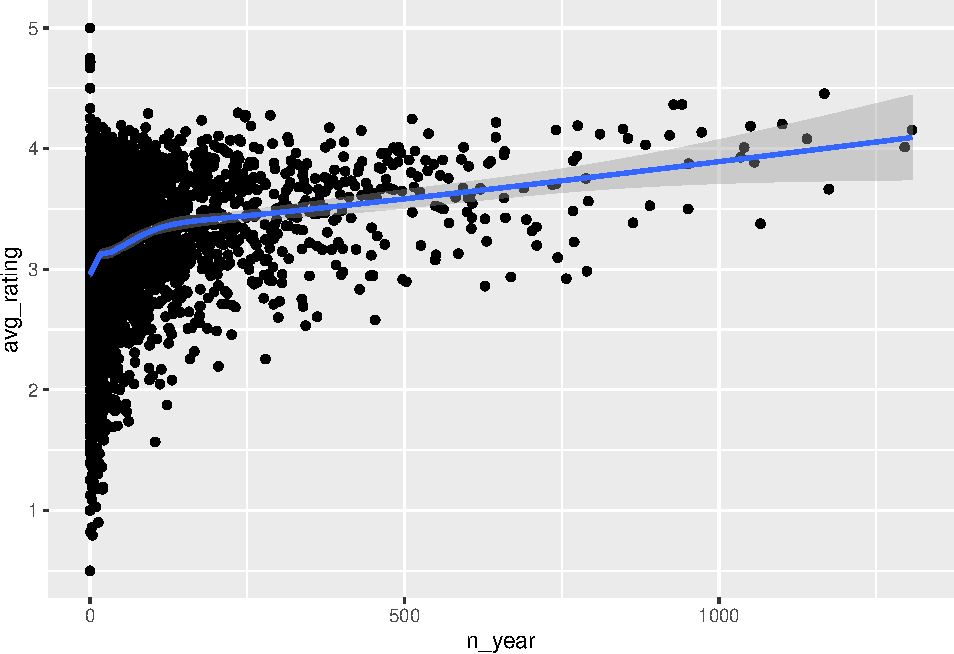
\includegraphics{figures/md_4-1.pdf}
\caption{Movies average ratings versus ratings per year post
1993\label{fig:movies_average_ratings_versus_ratings_per_year_post_1993}}
\end{figure}

\newpage

\textbf{Pre-1993 movies}\\
Compare Pre-1993 movies trend shown here in Figure
\ref{fig:movies_average_ratings_versus_ratings_per_year_pre_1993} Versus
Post-1993 movies trend in Figure
\ref{fig:movies_average_ratings_versus_ratings_per_year_post_1993}
above.

\begin{verbatim}
`geom_smooth()` using method = 'gam' and formula 'y ~ s(x, bs = "cs")'
\end{verbatim}

\begin{figure}
\centering
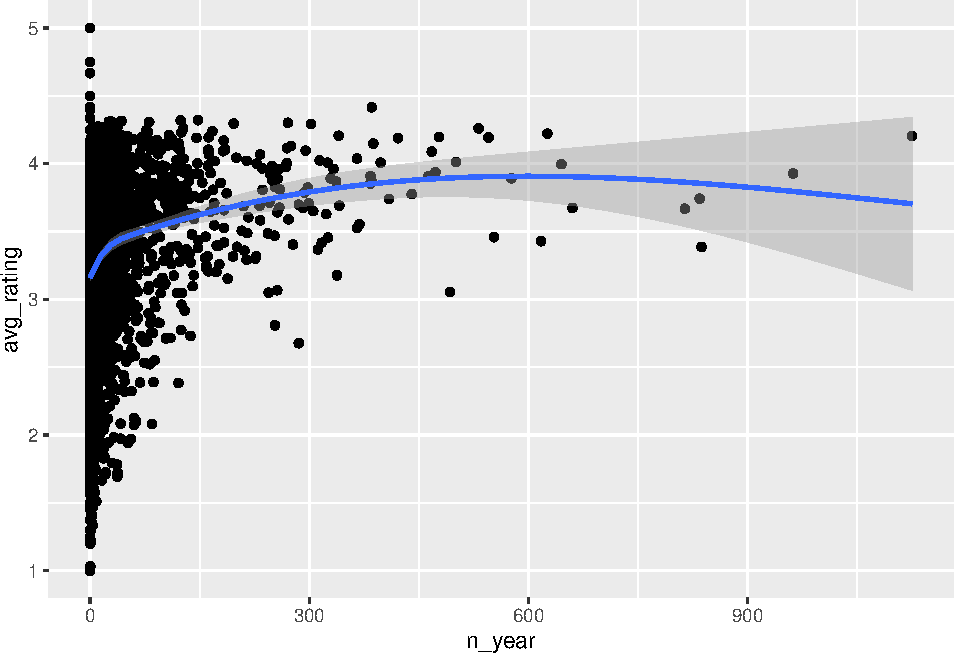
\includegraphics{figures/md_5-1.pdf}
\caption{Movies average ratings versus ratings per year pre
1993\label{fig:movies_average_ratings_versus_ratings_per_year_pre_1993}}
\end{figure}

\newpage

\hypertarget{movie-rating-date-time---a-closer-look}{%
\paragraph{Movie Rating Date-Time - a closer
look}\label{movie-rating-date-time---a-closer-look}}

The Movielens edx data Table \ref{tbl:movielens_data} also includes a
time stamp. This variable represents the time and date in which the
rating was provided. The units are seconds since January 1, 1970. We
create a new column date with the date named \emph{rating\_date} in
subsection \protect\hyperlink{modify_edx}{Modify edx} to get Table
\ref{tbl:movielens_edx_movie_release_date} .

We compute the average rating for each week and plot this average
against day. See Figure
\ref{fig:movies_average_ratings_for_each_week_versus_day} :

\begin{verbatim}
`geom_smooth()` using method = 'loess' and formula 'y ~ x'
\end{verbatim}

\begin{figure}
\centering
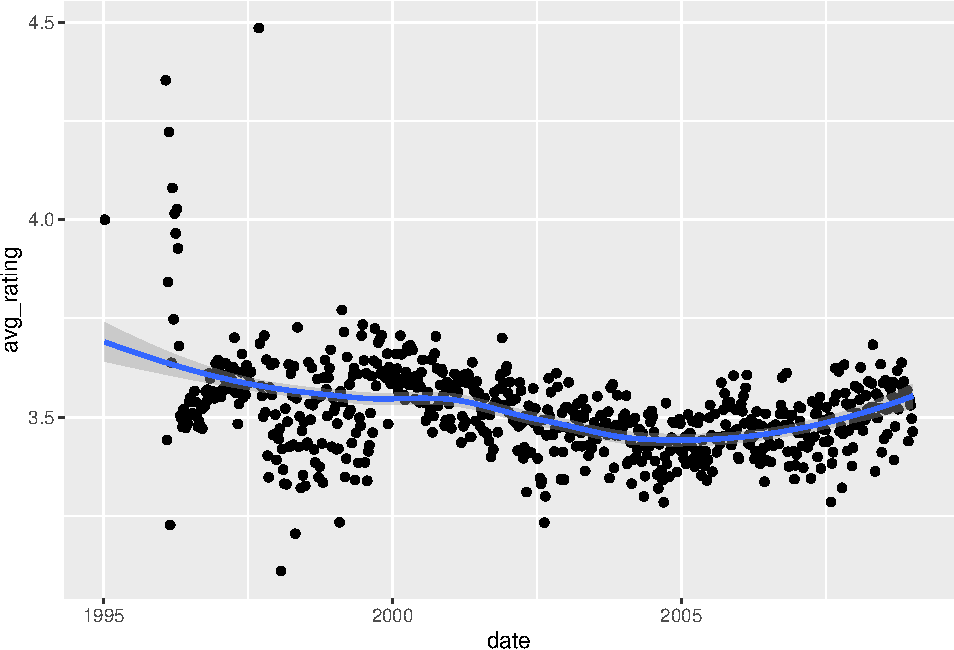
\includegraphics{figures/rd_1-1.pdf}
\caption{Movies average ratings for each week versus
day\label{fig:movies_average_ratings_for_each_week_versus_day}}
\end{figure}

The plot shows some evidence of a time effect. If we define \(d_{u,i}\)
as the day for user's \emph{u} rating of movie \emph{i}, then the
following model given by Equation \ref{eq:EqTimeEffect} is most
appropriate:

%
\refstepcounter{equations}
\par\noindent\textbf{equations \theequations. Equation \ref{eq:EqTimeEffect}}
\addcontentsline{equ}{equations}{\thesection. \protect\numberline{\theequations}Equation \ref{eq:EqTimeEffect}}\par

\label{eq:EqTimeEffect} \begin{equation}
Y_{u,i}=\mu+b_{i}+b_{u}+f(d_{u,i})+\epsilon_{u,i}\text{, with f a smooth function of }d_{u,i}
\end{equation}

\textbf{\emph{Modify edx}} Let's update the \textbf{\emph{edx}} table to
get Table \ref{tbl:movielens_edx_avg_rating_time_effect} below:

\begin{table}[H]

\caption{\label{tab:rd_2}Movielens edx data with average rating due to rating time effect\label{tbl:movielens_edx_avg_rating_time_effect}}
\centering
\fontsize{6}{8}\selectfont
\begin{tabular}[t]{rrrlllrlr}
\toprule
userId & movieId & rating & title & genres & rating\_date & movie\_dt & date & avg\_rating\\
\midrule
1 & 122 & 5 & Boomerang & Comedy|Romance & 1996-08-02 11:24:06 & 1992 & 1996-08-04 & 3.538801\\
1 & 185 & 5 & Net, The & Action|Crime|Thriller & 1996-08-02 10:58:45 & 1995 & 1996-08-04 & 3.538801\\
1 & 292 & 5 & Outbreak & Action|Drama|Sci-Fi|Thriller & 1996-08-02 10:57:01 & 1995 & 1996-08-04 & 3.538801\\
1 & 316 & 5 & Stargate & Action|Adventure|Sci-Fi & 1996-08-02 10:56:32 & 1994 & 1996-08-04 & 3.538801\\
1 & 329 & 5 & Star Trek: Generations & Action|Adventure|Drama|Sci-Fi & 1996-08-02 10:56:32 & 1994 & 1996-08-04 & 3.538801\\
\bottomrule
\end{tabular}
\end{table}

\textbf{TODO: Repeat above for validation data as well and somehow add
this to the modelling section}

\textbf{\emph{Modify validation}} We need to do the above
\textbf{\emph{avg\_rating\_time\_effect}} update for the validation data
as well. Let's update the \textbf{\emph{validation}} table to get Table
\ref{tbl:movielens_validation_avg_rating_time_effect} below:

\begin{table}[H]

\caption{\label{tab:rd_3}Movielens validation data with average rating due to rating time effect\label{tbl:movielens_validation_avg_rating_time_effect}}
\centering
\fontsize{6}{8}\selectfont
\begin{tabular}[t]{rrrlllrlr}
\toprule
userId & movieId & rating & title & genres & rating\_date & movie\_dt & date & avg\_rating\\
\midrule
1 & 231 & 5 & Dumb \& Dumber & Comedy & 1996-08-02 10:56:32 & 1994 & 1996-08-04 & 3.555820\\
1 & 480 & 5 & Jurassic Park & Action|Adventure|Sci-Fi|Thriller & 1996-08-02 11:00:53 & 1993 & 1996-08-04 & 3.555820\\
1 & 586 & 5 & Home Alone & Children|Comedy & 1996-08-02 11:07:48 & 1990 & 1996-08-04 & 3.555820\\
2 & 151 & 3 & Rob Roy & Action|Drama|Romance|War & 1997-07-07 03:34:10 & 1995 & 1997-07-06 & 3.606571\\
2 & 858 & 2 & Godfather, The & Crime|Drama & 1997-07-07 03:20:45 & 1972 & 1997-07-06 & 3.606571\\
\bottomrule
\end{tabular}
\end{table}

\newpage

\hypertarget{genres-combinations-per-movie---a-closer-look}{%
\paragraph{Genres combinations per movie - a closer
look}\label{genres-combinations-per-movie---a-closer-look}}

The movielens data Table \ref{tbl:movielens_edx_avg_rating_time_effect}
also has a genres column. This column includes every genre that applies
to the movie. Some movies fall under several genres. We define a
category as whatever combination appears in this column.

Here we keep only categories with more than 1,000 ratings. Then compute
the average and standard error for each category, and plot these as
error bar plots. See Figure \ref{fig:genres_error_bar_plots} :

\begin{figure}
\centering
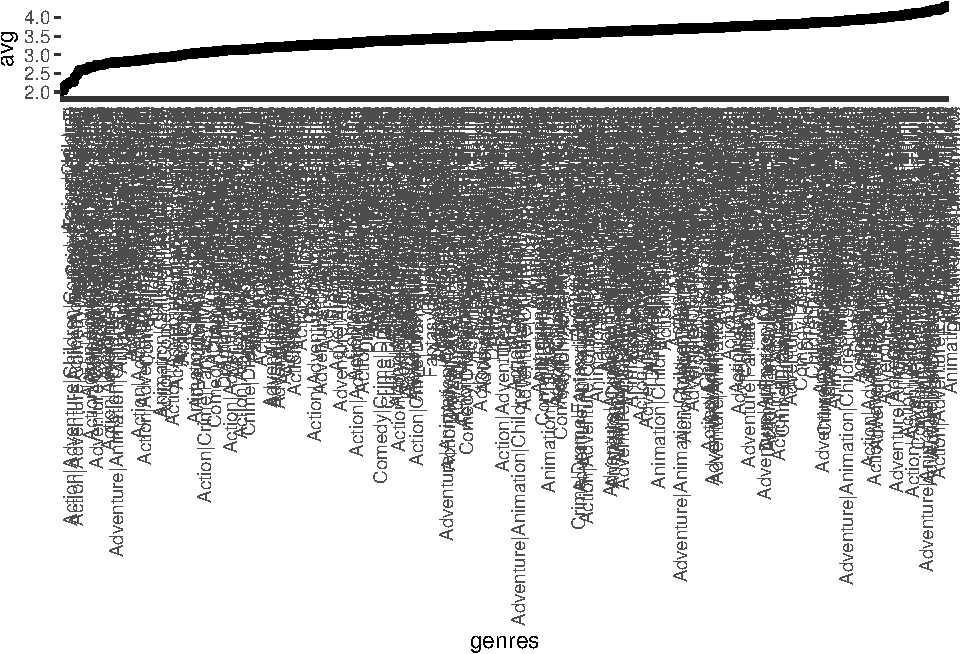
\includegraphics{figures/gnr-1.pdf}
\caption{Movies genres error bar
plots\label{fig:genres_error_bar_plots}}
\end{figure}

The plot shows strong evidence of a genre effect.

\newpage

\hypertarget{results}{%
\section{Results}\label{results}}

\begin{center}\rule{0.5\linewidth}{0.5pt}\end{center}

\newpage

\hypertarget{conclusion}{%
\section{Conclusion}\label{conclusion}}

\begin{center}\rule{0.5\linewidth}{0.5pt}\end{center}

\newpage

\hypertarget{appendix-all-code-for-this-report}{%
\section{Appendix: All code for this
report}\label{appendix-all-code-for-this-report}}

\begin{Shaded}
\begin{Highlighting}[]
\NormalTok{knitr}\SpecialCharTok{::}\NormalTok{knit\_hooks}\SpecialCharTok{$}\FunctionTok{set}\NormalTok{(}\AttributeTok{time\_it =} \FunctionTok{local}\NormalTok{(\{}
\NormalTok{  now }\OtherTok{\textless{}{-}} \ConstantTok{NULL}
  \ControlFlowTok{function}\NormalTok{(before, options) \{}
    \ControlFlowTok{if}\NormalTok{ (before) \{}
      \CommentTok{\# record the current time before each chunk}
\NormalTok{      now }\OtherTok{\textless{}\textless{}{-}} \FunctionTok{Sys.time}\NormalTok{()}
\NormalTok{    \} }\ControlFlowTok{else}\NormalTok{ \{}
      \CommentTok{\# calculate the time difference after a chunk}
\NormalTok{      res }\OtherTok{\textless{}{-}} \FunctionTok{difftime}\NormalTok{(}\FunctionTok{Sys.time}\NormalTok{(), now)}
      \CommentTok{\# return a character string to show the time}
      \CommentTok{\# paste("Time for this code chunk to run:", res)}
      \FunctionTok{paste}\NormalTok{(}\StringTok{"Time for the chunk"}\NormalTok{, options}\SpecialCharTok{$}\NormalTok{label, }\StringTok{"to run:"}\NormalTok{, res)}
\NormalTok{    \}}
\NormalTok{  \}}
\NormalTok{\}))}

\CommentTok{\# knitr::opts\_chunk$set(fig.pos = "!H", out.extra = "")}
\NormalTok{knitr}\SpecialCharTok{::}\NormalTok{opts\_chunk}\SpecialCharTok{$}\FunctionTok{set}\NormalTok{(}\AttributeTok{echo =} \ConstantTok{TRUE}\NormalTok{,}
                      \AttributeTok{fig.path =} \StringTok{"figures/"}\NormalTok{)}

\CommentTok{\# Beware, using the "time\_it" hook messes up fig.cap, \textbackslash{}label, \textbackslash{}ref}
\CommentTok{\# knitr::opts\_chunk$set(time\_it = TRUE)}
\CommentTok{\#knitr::opts\_chunk$set(eval = FALSE)}
  \FunctionTok{library}\NormalTok{(ggplot2)}
  \FunctionTok{library}\NormalTok{(kableExtra)}

\DocumentationTok{\#\#\#\#\#\#\#\#\#\#\#\#\#\#\#\#\#\#\#\#\#\#\#\#\#\#\#\#\#\#\#\#}
\CommentTok{\# Create edx set, validation set}
\DocumentationTok{\#\#\#\#\#\#\#\#\#\#\#\#\#\#\#\#\#\#\#\#\#\#\#\#\#\#\#\#\#\#\#\#}

\CommentTok{\# Note: this process could take a couple of minutes}

\ControlFlowTok{if}\NormalTok{(}\SpecialCharTok{!}\FunctionTok{require}\NormalTok{(tidyverse)) }\FunctionTok{install.packages}\NormalTok{(}\StringTok{"tidyverse"}\NormalTok{, }\AttributeTok{repos =} \StringTok{"http://cran.us.r{-}project.org"}\NormalTok{)}
\ControlFlowTok{if}\NormalTok{(}\SpecialCharTok{!}\FunctionTok{require}\NormalTok{(caret)) }\FunctionTok{install.packages}\NormalTok{(}\StringTok{"caret"}\NormalTok{, }\AttributeTok{repos =} \StringTok{"http://cran.us.r{-}project.org"}\NormalTok{)}
\ControlFlowTok{if}\NormalTok{(}\SpecialCharTok{!}\FunctionTok{require}\NormalTok{(data.table)) }\FunctionTok{install.packages}\NormalTok{(}\StringTok{"data.table"}\NormalTok{, }\AttributeTok{repos =} \StringTok{"http://cran.us.r{-}project.org"}\NormalTok{)}
\ControlFlowTok{if}\NormalTok{(}\SpecialCharTok{!}\FunctionTok{require}\NormalTok{(lubridate)) }\FunctionTok{install.packages}\NormalTok{(}\StringTok{"caret"}\NormalTok{, }\AttributeTok{repos =} \StringTok{"http://cran.us.r{-}project.org"}\NormalTok{)}
\ControlFlowTok{if}\NormalTok{(}\SpecialCharTok{!}\FunctionTok{require}\NormalTok{(groupdata2)) }\FunctionTok{install.packages}\NormalTok{(}\StringTok{"data.table"}\NormalTok{, }\AttributeTok{repos =} \StringTok{"http://cran.us.r{-}project.org"}\NormalTok{)}

\CommentTok{\# https://www.tidyverse.org/blog/2020/05/dplyr{-}1{-}0{-}0{-}last{-}minute{-}additions/}
\FunctionTok{options}\NormalTok{(}\AttributeTok{dplyr.summarise.inform =} \ConstantTok{FALSE}\NormalTok{)}

\CommentTok{\# MovieLens 10M dataset:}
\CommentTok{\# https://grouplens.org/datasets/movielens/10m/}
\CommentTok{\# http://files.grouplens.org/datasets/movielens/ml{-}10m{-}README.html}
\CommentTok{\# http://files.grouplens.org/datasets/movielens/ml{-}10m.zip}

\NormalTok{dl }\OtherTok{\textless{}{-}} \FunctionTok{tempfile}\NormalTok{()}
\FunctionTok{download.file}\NormalTok{(}\StringTok{"http://files.grouplens.org/datasets/movielens/ml{-}10m.zip"}\NormalTok{, dl)}

\NormalTok{ratings }\OtherTok{\textless{}{-}} \FunctionTok{fread}\NormalTok{(}\AttributeTok{text =} \FunctionTok{gsub}\NormalTok{(}\StringTok{"::"}\NormalTok{, }\StringTok{"}\SpecialCharTok{\textbackslash{}t}\StringTok{"}\NormalTok{, }\FunctionTok{readLines}\NormalTok{(}\FunctionTok{unzip}\NormalTok{(dl, }\StringTok{"ml{-}10M100K/ratings.dat"}\NormalTok{))),}
                 \AttributeTok{col.names =} \FunctionTok{c}\NormalTok{(}\StringTok{"userId"}\NormalTok{, }\StringTok{"movieId"}\NormalTok{, }\StringTok{"rating"}\NormalTok{, }\StringTok{"timestamp"}\NormalTok{))}

\NormalTok{movies }\OtherTok{\textless{}{-}} \FunctionTok{str\_split\_fixed}\NormalTok{(}\FunctionTok{readLines}\NormalTok{(}\FunctionTok{unzip}\NormalTok{(dl, }\StringTok{"ml{-}10M100K/movies.dat"}\NormalTok{)), }\StringTok{"}\SpecialCharTok{\textbackslash{}\textbackslash{}}\StringTok{::"}\NormalTok{, }\DecValTok{3}\NormalTok{)}
\FunctionTok{colnames}\NormalTok{(movies) }\OtherTok{\textless{}{-}} \FunctionTok{c}\NormalTok{(}\StringTok{"movieId"}\NormalTok{, }\StringTok{"title"}\NormalTok{, }\StringTok{"genres"}\NormalTok{)}
\NormalTok{movies }\OtherTok{\textless{}{-}} \FunctionTok{as.data.frame}\NormalTok{(movies) }\SpecialCharTok{\%\textgreater{}\%} \FunctionTok{mutate}\NormalTok{(}\AttributeTok{movieId =} \FunctionTok{as.numeric}\NormalTok{(movieId),}
                                           \AttributeTok{title =} \FunctionTok{as.character}\NormalTok{(title),}
                                           \AttributeTok{genres =} \FunctionTok{as.character}\NormalTok{(genres))}

\NormalTok{movielens }\OtherTok{\textless{}{-}} \FunctionTok{left\_join}\NormalTok{(ratings, movies, }\AttributeTok{by =} \StringTok{"movieId"}\NormalTok{)}

\CommentTok{\# Validation set will be 10\% of MovieLens data}
\FunctionTok{set.seed}\NormalTok{(}\DecValTok{1}\NormalTok{, }\AttributeTok{sample.kind=}\StringTok{"Rounding"}\NormalTok{)}
\CommentTok{\# if using R 3.5 or earlier, use \textasciigrave{}set.seed(1)\textasciigrave{} instead}
\NormalTok{test\_index }\OtherTok{\textless{}{-}} \FunctionTok{createDataPartition}\NormalTok{(}\AttributeTok{y =}\NormalTok{ movielens}\SpecialCharTok{$}\NormalTok{rating, }\AttributeTok{times =} \DecValTok{1}\NormalTok{, }\AttributeTok{p =} \FloatTok{0.1}\NormalTok{, }\AttributeTok{list =} \ConstantTok{FALSE}\NormalTok{)}
\NormalTok{edx }\OtherTok{\textless{}{-}}\NormalTok{ movielens[}\SpecialCharTok{{-}}\NormalTok{test\_index,]}
\NormalTok{temp }\OtherTok{\textless{}{-}}\NormalTok{ movielens[test\_index,]}

\CommentTok{\# Make sure userId and movieId in validation set are also in edx set}
\NormalTok{validation }\OtherTok{\textless{}{-}}\NormalTok{ temp }\SpecialCharTok{\%\textgreater{}\%}
  \FunctionTok{semi\_join}\NormalTok{(edx, }\AttributeTok{by =} \StringTok{"movieId"}\NormalTok{) }\SpecialCharTok{\%\textgreater{}\%}
  \FunctionTok{semi\_join}\NormalTok{(edx, }\AttributeTok{by =} \StringTok{"userId"}\NormalTok{)}

\CommentTok{\# Add rows removed from validation set back into edx set}
\NormalTok{removed }\OtherTok{\textless{}{-}} \FunctionTok{anti\_join}\NormalTok{(temp, validation)}
\NormalTok{edx }\OtherTok{\textless{}{-}} \FunctionTok{rbind}\NormalTok{(edx, removed)}

\FunctionTok{save}\NormalTok{(ratings, }\AttributeTok{file =} \StringTok{"rdas/ratings.rda"}\NormalTok{)}
\FunctionTok{save}\NormalTok{(movies, }\AttributeTok{file =} \StringTok{"rdas/movies.rda"}\NormalTok{)}
\FunctionTok{rm}\NormalTok{(dl, ratings, movies, test\_index, temp, movielens, removed)}

\FunctionTok{save}\NormalTok{(edx, }\AttributeTok{file =} \StringTok{"rdas/edx.rda"}\NormalTok{)}
\FunctionTok{save}\NormalTok{(validation, }\AttributeTok{file =} \StringTok{"rdas/validation.rda"}\NormalTok{)}
  \FunctionTok{kable}\NormalTok{(edx[}\DecValTok{1}\SpecialCharTok{:}\DecValTok{10}\NormalTok{,], }\StringTok{"latex"}\NormalTok{, }\AttributeTok{escape=}\ConstantTok{FALSE}\NormalTok{, }\AttributeTok{booktabs=}\ConstantTok{TRUE}\NormalTok{, }\AttributeTok{linesep=}\StringTok{""}\NormalTok{, }\AttributeTok{caption=}\StringTok{"Movielens data}\SpecialCharTok{\textbackslash{}\textbackslash{}}\StringTok{label\{tbl:movielens\_data\}"}\NormalTok{) }\SpecialCharTok{\%\textgreater{}\%}
    \FunctionTok{kable\_styling}\NormalTok{(}\AttributeTok{latex\_options=}\FunctionTok{c}\NormalTok{(}\StringTok{"HOLD\_position"}\NormalTok{), }\AttributeTok{font\_size=}\DecValTok{7}\NormalTok{)}
\NormalTok{unique\_u\_m\_g }\OtherTok{\textless{}{-}}\NormalTok{ edx }\SpecialCharTok{\%\textgreater{}\%} 
  \FunctionTok{summarize}\NormalTok{(}\AttributeTok{unique\_users =} \FunctionTok{n\_distinct}\NormalTok{(userId),}
            \AttributeTok{unique\_movies =} \FunctionTok{n\_distinct}\NormalTok{(movieId), }
            \AttributeTok{unique\_genres =} \FunctionTok{n\_distinct}\NormalTok{(genres))}

\FunctionTok{kable}\NormalTok{(unique\_u\_m\_g, }\StringTok{"latex"}\NormalTok{, }
      \AttributeTok{booktabs=}\ConstantTok{TRUE}\NormalTok{, }\AttributeTok{linesep=}\StringTok{""}\NormalTok{,}
      \AttributeTok{caption=}\StringTok{"Unique Users, Movies and Genres}\SpecialCharTok{\textbackslash{}\textbackslash{}}\StringTok{label\{tbl:uniq\_users\_movies\_genres\}"}\NormalTok{) }\SpecialCharTok{\%\textgreater{}\%}  \FunctionTok{kable\_styling}\NormalTok{(}\AttributeTok{latex\_options=}\FunctionTok{c}\NormalTok{(}\StringTok{"HOLD\_position"}\NormalTok{))}
\NormalTok{keep }\OtherTok{\textless{}{-}}\NormalTok{ edx }\SpecialCharTok{\%\textgreater{}\%}
\NormalTok{  dplyr}\SpecialCharTok{::}\FunctionTok{count}\NormalTok{(movieId) }\SpecialCharTok{\%\textgreater{}\%}
  \FunctionTok{top\_n}\NormalTok{(}\DecValTok{4}\NormalTok{) }\SpecialCharTok{\%\textgreater{}\%}
  \FunctionTok{pull}\NormalTok{(movieId)}
\NormalTok{tab }\OtherTok{\textless{}{-}}\NormalTok{ edx }\SpecialCharTok{\%\textgreater{}\%}
  \FunctionTok{filter}\NormalTok{(userId }\SpecialCharTok{\%in\%} \FunctionTok{c}\NormalTok{(}\DecValTok{13}\SpecialCharTok{:}\DecValTok{20}\NormalTok{)) }\SpecialCharTok{\%\textgreater{}\%} 
  \FunctionTok{filter}\NormalTok{(movieId }\SpecialCharTok{\%in\%}\NormalTok{ keep) }\SpecialCharTok{\%\textgreater{}\%} 
  \FunctionTok{select}\NormalTok{(userId, title, rating) }\SpecialCharTok{\%\textgreater{}\%} 
  \FunctionTok{spread}\NormalTok{(title, rating)}
  
\FunctionTok{kable}\NormalTok{(tab, }\StringTok{"latex"}\NormalTok{, }\AttributeTok{escape=}\ConstantTok{FALSE}\NormalTok{, }\AttributeTok{booktabs=}\ConstantTok{TRUE}\NormalTok{, }\AttributeTok{linesep=}\StringTok{""}\NormalTok{, }\AttributeTok{caption=}\StringTok{"Matrix of seven users and four movies}\SpecialCharTok{\textbackslash{}\textbackslash{}}\StringTok{label\{tbl:matrix\_seven\_users\_four\_movies\}"}\NormalTok{) }\SpecialCharTok{\%\textgreater{}\%}
    \FunctionTok{kable\_styling}\NormalTok{(}\AttributeTok{latex\_options=}\FunctionTok{c}\NormalTok{(}\StringTok{"HOLD\_position"}\NormalTok{), }\AttributeTok{font\_size=}\DecValTok{8}\NormalTok{)}
\NormalTok{users }\OtherTok{\textless{}{-}} \FunctionTok{sample}\NormalTok{(}\FunctionTok{unique}\NormalTok{(edx}\SpecialCharTok{$}\NormalTok{userId), }\DecValTok{100}\NormalTok{)}
\NormalTok{rafalib}\SpecialCharTok{::}\FunctionTok{mypar}\NormalTok{()}
\NormalTok{edx }\SpecialCharTok{\%\textgreater{}\%} \FunctionTok{filter}\NormalTok{(userId }\SpecialCharTok{\%in\%}\NormalTok{ users) }\SpecialCharTok{\%\textgreater{}\%} 
  \FunctionTok{select}\NormalTok{(userId, movieId, rating) }\SpecialCharTok{\%\textgreater{}\%}
  \FunctionTok{mutate}\NormalTok{(}\AttributeTok{rating =} \DecValTok{1}\NormalTok{) }\SpecialCharTok{\%\textgreater{}\%}
  \FunctionTok{spread}\NormalTok{(movieId, rating) }\SpecialCharTok{\%\textgreater{}\%} \FunctionTok{select}\NormalTok{(}\FunctionTok{sample}\NormalTok{(}\FunctionTok{ncol}\NormalTok{(.), }\DecValTok{100}\NormalTok{)) }\SpecialCharTok{\%\textgreater{}\%} 
  \FunctionTok{as.matrix}\NormalTok{() }\SpecialCharTok{\%\textgreater{}\%} \FunctionTok{t}\NormalTok{(.) }\SpecialCharTok{\%\textgreater{}\%}
  \FunctionTok{image}\NormalTok{(}\DecValTok{1}\SpecialCharTok{:}\DecValTok{100}\NormalTok{, }\DecValTok{1}\SpecialCharTok{:}\DecValTok{100}\NormalTok{,. , }\AttributeTok{xlab=}\StringTok{"Movies"}\NormalTok{, }\AttributeTok{ylab=}\StringTok{"Users"}\NormalTok{)}
\FunctionTok{abline}\NormalTok{(}\AttributeTok{h=}\DecValTok{0}\SpecialCharTok{:}\DecValTok{100}\FloatTok{+0.5}\NormalTok{, }\AttributeTok{v=}\DecValTok{0}\SpecialCharTok{:}\DecValTok{100}\FloatTok{+0.5}\NormalTok{, }\AttributeTok{col =} \StringTok{"grey"}\NormalTok{)}
\NormalTok{edx }\SpecialCharTok{\%\textgreater{}\%} 
\NormalTok{  dplyr}\SpecialCharTok{::}\FunctionTok{count}\NormalTok{(movieId) }\SpecialCharTok{\%\textgreater{}\%} 
  \FunctionTok{ggplot}\NormalTok{(}\FunctionTok{aes}\NormalTok{(n)) }\SpecialCharTok{+} 
  \FunctionTok{geom\_histogram}\NormalTok{(}\AttributeTok{bins =} \DecValTok{30}\NormalTok{, }\AttributeTok{color =} \StringTok{"black"}\NormalTok{) }\SpecialCharTok{+} 
  \FunctionTok{scale\_x\_log10}\NormalTok{() }\SpecialCharTok{+}  \CommentTok{\# try with and without this line}
  \FunctionTok{ggtitle}\NormalTok{(}\StringTok{"Movies"}\NormalTok{)}
\NormalTok{edx }\SpecialCharTok{\%\textgreater{}\%}
\NormalTok{  dplyr}\SpecialCharTok{::}\FunctionTok{count}\NormalTok{(userId) }\SpecialCharTok{\%\textgreater{}\%} 
  \FunctionTok{ggplot}\NormalTok{(}\FunctionTok{aes}\NormalTok{(n)) }\SpecialCharTok{+} 
  \FunctionTok{geom\_histogram}\NormalTok{(}\AttributeTok{bins =} \DecValTok{30}\NormalTok{, }\AttributeTok{color =} \StringTok{"black"}\NormalTok{) }\SpecialCharTok{+} 
  \FunctionTok{scale\_x\_log10}\NormalTok{() }\SpecialCharTok{+} \CommentTok{\# try with and without this line}
  \FunctionTok{ggtitle}\NormalTok{(}\StringTok{"Users"}\NormalTok{)}

\FunctionTok{rm}\NormalTok{(tab,keep,unique\_u\_m\_g,users)}
\NormalTok{edx\_dt }\OtherTok{\textless{}{-}}\NormalTok{ edx }\SpecialCharTok{\%\textgreater{}\%} 
  \FunctionTok{mutate}\NormalTok{(}\AttributeTok{rating\_date =} \FunctionTok{as\_datetime}\NormalTok{(timestamp)) }\SpecialCharTok{\%\textgreater{}\%} 
  \FunctionTok{select}\NormalTok{(}\SpecialCharTok{{-}}\NormalTok{timestamp)}
\FunctionTok{rm}\NormalTok{(edx)}

\FunctionTok{kable}\NormalTok{(edx\_dt[}\DecValTok{1}\SpecialCharTok{:}\DecValTok{5}\NormalTok{,], }\StringTok{"latex"}\NormalTok{, }\AttributeTok{escape=}\ConstantTok{TRUE}\NormalTok{, }\AttributeTok{booktabs=}\ConstantTok{TRUE}\NormalTok{, }\AttributeTok{linesep=}\StringTok{""}\NormalTok{, }\AttributeTok{caption=}\StringTok{"Movielens edx data with rating date{-}time}\SpecialCharTok{\textbackslash{}\textbackslash{}}\StringTok{label\{tbl:movielens\_edx\_data\_rating\_date\}"}\NormalTok{) }\SpecialCharTok{\%\textgreater{}\%}
    \FunctionTok{kable\_styling}\NormalTok{(}\AttributeTok{latex\_options=}\FunctionTok{c}\NormalTok{(}\StringTok{"HOLD\_position"}\NormalTok{), }\AttributeTok{font\_size=}\DecValTok{8}\NormalTok{)}
\NormalTok{td }\OtherTok{\textless{}{-}}\NormalTok{ edx\_dt}\SpecialCharTok{$}\NormalTok{title}
\NormalTok{movie\_dt }\OtherTok{\textless{}{-}} \FunctionTok{str\_extract}\NormalTok{(td, }\StringTok{"}\SpecialCharTok{\textbackslash{}\textbackslash{}}\StringTok{([0{-}9]\{4\}}\SpecialCharTok{\textbackslash{}\textbackslash{}}\StringTok{)$"}\NormalTok{) }\SpecialCharTok{\%\textgreater{}\%}
  \FunctionTok{str\_extract}\NormalTok{(}\StringTok{"[0{-}9]\{4\}"}\NormalTok{)}
\NormalTok{title\_o }\OtherTok{\textless{}{-}} \FunctionTok{str\_replace}\NormalTok{(td, }\StringTok{"}\SpecialCharTok{\textbackslash{}\textbackslash{}}\StringTok{([0{-}9]\{4\}}\SpecialCharTok{\textbackslash{}\textbackslash{}}\StringTok{)$"}\NormalTok{, }\StringTok{""}\NormalTok{)}
\NormalTok{edx\_md }\OtherTok{\textless{}{-}}\NormalTok{ edx\_dt }\SpecialCharTok{\%\textgreater{}\%} \FunctionTok{mutate}\NormalTok{(}\AttributeTok{title=}\NormalTok{title\_o, }\AttributeTok{movie\_dt=}\FunctionTok{as.numeric}\NormalTok{(movie\_dt))}
\FunctionTok{rm}\NormalTok{(td,movie\_dt,title\_o,edx\_dt)}
\FunctionTok{save}\NormalTok{(edx\_md, }\AttributeTok{file =} \StringTok{"rdas/edx\_md.rda"}\NormalTok{)}

\FunctionTok{kable}\NormalTok{(edx\_md[}\DecValTok{1}\SpecialCharTok{:}\DecValTok{5}\NormalTok{,], }\StringTok{"latex"}\NormalTok{, }\AttributeTok{escape=}\ConstantTok{TRUE}\NormalTok{, }\AttributeTok{booktabs=}\ConstantTok{TRUE}\NormalTok{, }\AttributeTok{linesep=}\StringTok{""}\NormalTok{, }\AttributeTok{caption=}\StringTok{"Movielens edx data with movie release date}\SpecialCharTok{\textbackslash{}\textbackslash{}}\StringTok{label\{tbl:movielens\_edx\_movie\_release\_date\}"}\NormalTok{) }\SpecialCharTok{\%\textgreater{}\%}
    \FunctionTok{kable\_styling}\NormalTok{(}\AttributeTok{latex\_options=}\FunctionTok{c}\NormalTok{(}\StringTok{"HOLD\_position"}\NormalTok{), }\AttributeTok{font\_size=}\DecValTok{8}\NormalTok{)}
\NormalTok{validation\_dt }\OtherTok{\textless{}{-}}\NormalTok{ validation }\SpecialCharTok{\%\textgreater{}\%} 
  \FunctionTok{mutate}\NormalTok{(}\AttributeTok{rating\_date =} \FunctionTok{as\_datetime}\NormalTok{(timestamp)) }\SpecialCharTok{\%\textgreater{}\%} 
  \FunctionTok{select}\NormalTok{(}\SpecialCharTok{{-}}\NormalTok{timestamp)}
\FunctionTok{rm}\NormalTok{(validation)}

\FunctionTok{kable}\NormalTok{(validation\_dt[}\DecValTok{1}\SpecialCharTok{:}\DecValTok{5}\NormalTok{,], }\StringTok{"latex"}\NormalTok{, }\AttributeTok{escape=}\ConstantTok{TRUE}\NormalTok{, }\AttributeTok{booktabs=}\ConstantTok{TRUE}\NormalTok{, }\AttributeTok{linesep=}\StringTok{""}\NormalTok{, }\AttributeTok{caption=}\StringTok{"Movielens validation data with rating date{-}time}\SpecialCharTok{\textbackslash{}\textbackslash{}}\StringTok{label\{tbl:movielens\_val\_data\_rating\_date\}"}\NormalTok{) }\SpecialCharTok{\%\textgreater{}\%}
    \FunctionTok{kable\_styling}\NormalTok{(}\AttributeTok{latex\_options=}\FunctionTok{c}\NormalTok{(}\StringTok{"HOLD\_position"}\NormalTok{), }\AttributeTok{font\_size=}\DecValTok{8}\NormalTok{)}
\NormalTok{td }\OtherTok{\textless{}{-}}\NormalTok{ validation\_dt}\SpecialCharTok{$}\NormalTok{title}
\NormalTok{movie\_dt }\OtherTok{\textless{}{-}} \FunctionTok{str\_extract}\NormalTok{(td, }\StringTok{"}\SpecialCharTok{\textbackslash{}\textbackslash{}}\StringTok{([0{-}9]\{4\}}\SpecialCharTok{\textbackslash{}\textbackslash{}}\StringTok{)$"}\NormalTok{) }\SpecialCharTok{\%\textgreater{}\%} 
  \FunctionTok{str\_extract}\NormalTok{(}\StringTok{"[0{-}9]\{4\}"}\NormalTok{)}
\NormalTok{title\_o }\OtherTok{\textless{}{-}} \FunctionTok{str\_replace}\NormalTok{(td, }\StringTok{"}\SpecialCharTok{\textbackslash{}\textbackslash{}}\StringTok{([0{-}9]\{4\}}\SpecialCharTok{\textbackslash{}\textbackslash{}}\StringTok{)$"}\NormalTok{, }\StringTok{""}\NormalTok{)}
\NormalTok{validation\_md }\OtherTok{\textless{}{-}}\NormalTok{ validation\_dt }\SpecialCharTok{\%\textgreater{}\%} \FunctionTok{mutate}\NormalTok{(}\AttributeTok{title=}\NormalTok{title\_o, }\AttributeTok{movie\_dt=}\FunctionTok{as.numeric}\NormalTok{(movie\_dt))}
\FunctionTok{rm}\NormalTok{(td,movie\_dt,title\_o,validation\_dt)}
\FunctionTok{save}\NormalTok{(validation\_md, }\AttributeTok{file =} \StringTok{"rdas/validation\_md.rda"}\NormalTok{)}

\FunctionTok{kable}\NormalTok{(validation\_md[}\DecValTok{1}\SpecialCharTok{:}\DecValTok{5}\NormalTok{,], }\StringTok{"latex"}\NormalTok{, }\AttributeTok{escape=}\ConstantTok{TRUE}\NormalTok{, }\AttributeTok{booktabs=}\ConstantTok{TRUE}\NormalTok{, }\AttributeTok{linesep=}\StringTok{""}\NormalTok{, }\AttributeTok{caption=}\StringTok{"Movielens validation data with movie release date}\SpecialCharTok{\textbackslash{}\textbackslash{}}\StringTok{label\{tbl:movielens\_val\_movie\_release\_date\}"}\NormalTok{) }\SpecialCharTok{\%\textgreater{}\%}
    \FunctionTok{kable\_styling}\NormalTok{(}\AttributeTok{latex\_options=}\FunctionTok{c}\NormalTok{(}\StringTok{"HOLD\_position"}\NormalTok{), }\AttributeTok{font\_size=}\DecValTok{8}\NormalTok{)}

\CommentTok{\# rm(validation\_md)}
\NormalTok{ratings\_m\_y }\OtherTok{\textless{}{-}}\NormalTok{ edx\_md }\SpecialCharTok{\%\textgreater{}\%}
  \FunctionTok{group\_by}\NormalTok{(movieId) }\SpecialCharTok{\%\textgreater{}\%}
  \FunctionTok{summarize}\NormalTok{(}\AttributeTok{n =} \FunctionTok{n\_distinct}\NormalTok{(userId), }\AttributeTok{year =} \FunctionTok{as.character}\NormalTok{(}\FunctionTok{first}\NormalTok{(movie\_dt))) }\SpecialCharTok{\%\textgreater{}\%} 
  \FunctionTok{mutate}\NormalTok{(}\AttributeTok{sqrt\_n=}\FunctionTok{sqrt}\NormalTok{(n)) }\SpecialCharTok{\%\textgreater{}\%} 
  \FunctionTok{group\_by}\NormalTok{(year) }\SpecialCharTok{\%\textgreater{}\%} 
  \FunctionTok{mutate}\NormalTok{(}\AttributeTok{r\_median=}\FunctionTok{median}\NormalTok{(sqrt\_n)) }\SpecialCharTok{\%\textgreater{}\%} \FunctionTok{select}\NormalTok{(year,r\_median) }\SpecialCharTok{\%\textgreater{}\%} 
  \FunctionTok{unique}\NormalTok{() }\SpecialCharTok{\%\textgreater{}\%} \FunctionTok{arrange}\NormalTok{(}\FunctionTok{desc}\NormalTok{(r\_median))}

\CommentTok{\# min(edx\_md$movie\_dt)}
\CommentTok{\# \# [1] 1915}
\CommentTok{\# max(edx\_md$movie\_dt)}
\CommentTok{\# \# [1] 2008}

\CommentTok{\# View(ratings\_m\_y)}
\FunctionTok{ggplot}\NormalTok{(}\AttributeTok{data=}\NormalTok{ratings\_m\_y, }\FunctionTok{aes}\NormalTok{(}\AttributeTok{x=}\NormalTok{year, }\AttributeTok{y=}\NormalTok{r\_median) ) }\SpecialCharTok{+} 
  \FunctionTok{geom\_point}\NormalTok{( }\AttributeTok{size=}\DecValTok{1}\NormalTok{, }\AttributeTok{colour=}\StringTok{"\#000080"}\NormalTok{ ) }\SpecialCharTok{+} 
  \FunctionTok{theme\_light}\NormalTok{(}\AttributeTok{base\_size=}\DecValTok{8}\NormalTok{) }\SpecialCharTok{+} 
  \CommentTok{\# labs(title="", x="\textbackslash{}nyear", y="r\_median\textbackslash{}n") + }
  \FunctionTok{scale\_x\_discrete}\NormalTok{(}\AttributeTok{breaks=}\FunctionTok{seq}\NormalTok{(}\FunctionTok{min}\NormalTok{(edx\_md}\SpecialCharTok{$}\NormalTok{movie\_dt),}\FunctionTok{max}\NormalTok{(edx\_md}\SpecialCharTok{$}\NormalTok{movie\_dt),}\AttributeTok{by=}\DecValTok{2}\NormalTok{)) }\SpecialCharTok{+} 
  \FunctionTok{theme}\NormalTok{(}\AttributeTok{axis.text.x =} \FunctionTok{element\_text}\NormalTok{(}\AttributeTok{angle =} \DecValTok{90}\NormalTok{, }\AttributeTok{hjust =} \DecValTok{1}\NormalTok{))}

\NormalTok{spline\_int }\OtherTok{\textless{}{-}} \FunctionTok{as.data.frame}\NormalTok{(}\FunctionTok{spline}\NormalTok{(ratings\_m\_y}\SpecialCharTok{$}\NormalTok{year, ratings\_m\_y}\SpecialCharTok{$}\NormalTok{r\_median))}

\FunctionTok{ggplot}\NormalTok{(}\AttributeTok{data=}\NormalTok{ratings\_m\_y, }\FunctionTok{aes}\NormalTok{(}\AttributeTok{x=}\NormalTok{year, }\AttributeTok{y=}\NormalTok{r\_median) ) }\SpecialCharTok{+}
  \FunctionTok{geom\_point}\NormalTok{(}\AttributeTok{data =}\NormalTok{ spline\_int, }\FunctionTok{aes}\NormalTok{(}\AttributeTok{x =}\NormalTok{ x, }\AttributeTok{y =}\NormalTok{ y)) }\SpecialCharTok{+}
  \FunctionTok{geom\_line}\NormalTok{(}\AttributeTok{data =}\NormalTok{ spline\_int, }\FunctionTok{aes}\NormalTok{(}\AttributeTok{x =}\NormalTok{ x, }\AttributeTok{y =}\NormalTok{ y)) }\SpecialCharTok{+}
  \FunctionTok{theme\_light}\NormalTok{(}\AttributeTok{base\_size=}\DecValTok{8}\NormalTok{) }\SpecialCharTok{+}
  \CommentTok{\# scale\_x\_discrete(breaks=seq(min(edx\_md$movie\_dt),max(edx\_md$movie\_dt),by=2)) +}
  \FunctionTok{theme}\NormalTok{(}\AttributeTok{axis.text.x =} \FunctionTok{element\_text}\NormalTok{(}\AttributeTok{angle =} \DecValTok{90}\NormalTok{, }\AttributeTok{hjust =} \DecValTok{1}\NormalTok{))}

\FunctionTok{rm}\NormalTok{(ratings\_m\_y)}

\NormalTok{res2 }\OtherTok{\textless{}{-}}\NormalTok{ edx\_md }\SpecialCharTok{\%\textgreater{}\%}
  \FunctionTok{filter}\NormalTok{(movie\_dt }\SpecialCharTok{\textgreater{}=} \DecValTok{1991}\NormalTok{) }\SpecialCharTok{\%\textgreater{}\%}
  \FunctionTok{group\_by}\NormalTok{(movieId) }\SpecialCharTok{\%\textgreater{}\%}
  \CommentTok{\# summarize(avg\_rating = mean(rating), n = n(), title=title[1], years=2018 {-} min(movie\_dt)) \%\textgreater{}\% }
  \FunctionTok{summarize}\NormalTok{(}\AttributeTok{avg\_rating =} \FunctionTok{mean}\NormalTok{(rating), }\AttributeTok{n =} \FunctionTok{n}\NormalTok{(), }\AttributeTok{title=}\NormalTok{title[}\DecValTok{1}\NormalTok{], }\AttributeTok{years=}\DecValTok{2018} \SpecialCharTok{{-}} \FunctionTok{first}\NormalTok{(movie\_dt)) }\SpecialCharTok{\%\textgreater{}\%}
  \FunctionTok{mutate}\NormalTok{(}\AttributeTok{n\_year =}\NormalTok{ n }\SpecialCharTok{/}\NormalTok{ years) }\SpecialCharTok{\%\textgreater{}\%}
  \FunctionTok{top\_n}\NormalTok{(}\DecValTok{25}\NormalTok{, n\_year) }\SpecialCharTok{\%\textgreater{}\%}
  \FunctionTok{arrange}\NormalTok{(}\FunctionTok{desc}\NormalTok{(n\_year))}

\CommentTok{\# qplot(res2$years,res2$n)}
\FunctionTok{ggplot}\NormalTok{(res2,}\FunctionTok{aes}\NormalTok{(years,n)) }\SpecialCharTok{+} 
  \FunctionTok{geom\_line}\NormalTok{() }\SpecialCharTok{+} 
  \FunctionTok{geom\_smooth}\NormalTok{() }\SpecialCharTok{+} 
  \FunctionTok{geom\_vline}\NormalTok{(}\AttributeTok{xintercept =} \DecValTok{25}\NormalTok{) }\SpecialCharTok{+} \CommentTok{\# 1993}
  \FunctionTok{geom\_vline}\NormalTok{(}\AttributeTok{xintercept =} \DecValTok{27}\NormalTok{) }\CommentTok{\# 1991}
\FunctionTok{rm}\NormalTok{(res2)}
\NormalTok{res2\_1993\_plus }\OtherTok{\textless{}{-}}\NormalTok{ edx\_md }\SpecialCharTok{\%\textgreater{}\%}
  \FunctionTok{filter}\NormalTok{(movie\_dt }\SpecialCharTok{\textgreater{}=} \DecValTok{1993}\NormalTok{) }\SpecialCharTok{\%\textgreater{}\%}
  \FunctionTok{group\_by}\NormalTok{(movieId) }\SpecialCharTok{\%\textgreater{}\%}
  \CommentTok{\# summarize(avg\_rating = mean(rating), n = n(), title=title[1], years=2018 {-} min(movie\_dt)) \%\textgreater{}\% }
  \FunctionTok{summarize}\NormalTok{(}\AttributeTok{avg\_rating =} \FunctionTok{mean}\NormalTok{(rating), }\AttributeTok{n =} \FunctionTok{n}\NormalTok{(), }\AttributeTok{title=}\NormalTok{title[}\DecValTok{1}\NormalTok{], }\AttributeTok{years=}\DecValTok{2018} \SpecialCharTok{{-}} \FunctionTok{first}\NormalTok{(movie\_dt)) }\SpecialCharTok{\%\textgreater{}\%} 
  \FunctionTok{mutate}\NormalTok{(}\AttributeTok{n\_year =}\NormalTok{ n }\SpecialCharTok{/}\NormalTok{ years) }\SpecialCharTok{\%\textgreater{}\%}
  \FunctionTok{top\_n}\NormalTok{(}\DecValTok{25}\NormalTok{, n\_year) }\SpecialCharTok{\%\textgreater{}\%}
  \FunctionTok{arrange}\NormalTok{(}\FunctionTok{desc}\NormalTok{(n\_year))}
\CommentTok{\# qplot(res2\_1993\_plus$years,res2\_1993\_plus$n)}
\FunctionTok{ggplot}\NormalTok{(res2\_1993\_plus,}\FunctionTok{aes}\NormalTok{(years,n)) }\SpecialCharTok{+} 
  \FunctionTok{geom\_line}\NormalTok{() }\SpecialCharTok{+} 
  \FunctionTok{geom\_smooth}\NormalTok{() }\SpecialCharTok{+} 
  \FunctionTok{geom\_vline}\NormalTok{(}\AttributeTok{xintercept =} \DecValTok{25}\NormalTok{) }\CommentTok{\# 1993}

\FunctionTok{rm}\NormalTok{(res2\_1993\_plus)}
\NormalTok{res3 }\OtherTok{\textless{}{-}}\NormalTok{ edx\_md }\SpecialCharTok{\%\textgreater{}\%}
  \FunctionTok{filter}\NormalTok{(movie\_dt }\SpecialCharTok{\textgreater{}=} \DecValTok{1993}\NormalTok{) }\SpecialCharTok{\%\textgreater{}\%}
  \FunctionTok{group\_by}\NormalTok{(movieId) }\SpecialCharTok{\%\textgreater{}\%}
  \FunctionTok{summarize}\NormalTok{(}\AttributeTok{avg\_rating =} \FunctionTok{mean}\NormalTok{(rating), }\AttributeTok{n =} \FunctionTok{n}\NormalTok{(), }\AttributeTok{title=}\NormalTok{title[}\DecValTok{1}\NormalTok{], }\AttributeTok{years=}\DecValTok{2018} \SpecialCharTok{{-}} \FunctionTok{min}\NormalTok{(movie\_dt)) }\SpecialCharTok{\%\textgreater{}\%}
  \FunctionTok{mutate}\NormalTok{(}\AttributeTok{n\_year =}\NormalTok{ n }\SpecialCharTok{/}\NormalTok{ years)}
\NormalTok{res3 }\SpecialCharTok{\%\textgreater{}\%} 
  \FunctionTok{group\_by}\NormalTok{(}\FunctionTok{round}\NormalTok{(n\_year)) }\SpecialCharTok{\%\textgreater{}\%} 
  \FunctionTok{ggplot}\NormalTok{(}\FunctionTok{aes}\NormalTok{(n\_year,avg\_rating)) }\SpecialCharTok{+} \FunctionTok{geom\_point}\NormalTok{() }\SpecialCharTok{+} \FunctionTok{geom\_smooth}\NormalTok{()}

\FunctionTok{rm}\NormalTok{(res3)}
\NormalTok{res3\_b }\OtherTok{\textless{}{-}}\NormalTok{ edx\_md }\SpecialCharTok{\%\textgreater{}\%}
  \FunctionTok{filter}\NormalTok{(movie\_dt }\SpecialCharTok{\textless{}} \DecValTok{1993}\NormalTok{) }\SpecialCharTok{\%\textgreater{}\%}
  \FunctionTok{group\_by}\NormalTok{(movieId) }\SpecialCharTok{\%\textgreater{}\%}
  \FunctionTok{summarize}\NormalTok{(}\AttributeTok{avg\_rating =} \FunctionTok{mean}\NormalTok{(rating), }\AttributeTok{n =} \FunctionTok{n}\NormalTok{(), }\AttributeTok{title=}\NormalTok{title[}\DecValTok{1}\NormalTok{], }\AttributeTok{years=}\DecValTok{2018} \SpecialCharTok{{-}} \FunctionTok{min}\NormalTok{(movie\_dt)) }\SpecialCharTok{\%\textgreater{}\%}
  \FunctionTok{mutate}\NormalTok{(}\AttributeTok{n\_year =}\NormalTok{ n }\SpecialCharTok{/}\NormalTok{ years)}
\NormalTok{res3\_b }\SpecialCharTok{\%\textgreater{}\%} 
  \FunctionTok{group\_by}\NormalTok{(}\FunctionTok{round}\NormalTok{(n\_year)) }\SpecialCharTok{\%\textgreater{}\%} 
  \FunctionTok{ggplot}\NormalTok{(}\FunctionTok{aes}\NormalTok{(n\_year,avg\_rating)) }\SpecialCharTok{+} \FunctionTok{geom\_point}\NormalTok{() }\SpecialCharTok{+} \FunctionTok{geom\_smooth}\NormalTok{()}

\FunctionTok{rm}\NormalTok{(res3\_b)}
\NormalTok{edx\_md }\SpecialCharTok{\%\textgreater{}\%} \FunctionTok{mutate}\NormalTok{(}\AttributeTok{date =} \FunctionTok{round\_date}\NormalTok{(rating\_date, }\AttributeTok{unit =} \StringTok{"week"}\NormalTok{)) }\SpecialCharTok{\%\textgreater{}\%}
  \FunctionTok{group\_by}\NormalTok{(date) }\SpecialCharTok{\%\textgreater{}\%}
  \FunctionTok{summarize}\NormalTok{(}\AttributeTok{avg\_rating =} \FunctionTok{mean}\NormalTok{(rating)) }\SpecialCharTok{\%\textgreater{}\%}
  \FunctionTok{ggplot}\NormalTok{(}\FunctionTok{aes}\NormalTok{(date, avg\_rating)) }\SpecialCharTok{+}
  \FunctionTok{geom\_point}\NormalTok{() }\SpecialCharTok{+}
  \FunctionTok{geom\_smooth}\NormalTok{()}
\NormalTok{edx\_md }\OtherTok{\textless{}{-}}\NormalTok{ edx\_md }\SpecialCharTok{\%\textgreater{}\%} \FunctionTok{mutate}\NormalTok{(}\AttributeTok{date =} \FunctionTok{round\_date}\NormalTok{(rating\_date, }\AttributeTok{unit =} \StringTok{"week"}\NormalTok{)) }\SpecialCharTok{\%\textgreater{}\%}
  \FunctionTok{group\_by}\NormalTok{(date) }\SpecialCharTok{\%\textgreater{}\%}
  \FunctionTok{mutate}\NormalTok{(}\AttributeTok{avg\_rating =} \FunctionTok{mean}\NormalTok{(rating)) }\SpecialCharTok{\%\textgreater{}\%} \FunctionTok{ungroup}\NormalTok{()}
\FunctionTok{save}\NormalTok{(edx\_md, }\AttributeTok{file =} \StringTok{"rdas/edx\_md.rda"}\NormalTok{)}

\FunctionTok{kable}\NormalTok{(edx\_md[}\DecValTok{1}\SpecialCharTok{:}\DecValTok{5}\NormalTok{,], }\StringTok{"latex"}\NormalTok{, }\AttributeTok{escape=}\ConstantTok{TRUE}\NormalTok{, }\AttributeTok{booktabs=}\ConstantTok{TRUE}\NormalTok{, }\AttributeTok{linesep=}\StringTok{""}\NormalTok{, }\AttributeTok{caption=}\StringTok{"Movielens edx data with average rating due to rating time effect}\SpecialCharTok{\textbackslash{}\textbackslash{}}\StringTok{label\{tbl:movielens\_edx\_avg\_rating\_time\_effect\}"}\NormalTok{) }\SpecialCharTok{\%\textgreater{}\%}
    \FunctionTok{kable\_styling}\NormalTok{(}\AttributeTok{latex\_options=}\FunctionTok{c}\NormalTok{(}\StringTok{"HOLD\_position"}\NormalTok{), }\AttributeTok{font\_size=}\DecValTok{6}\NormalTok{)}
\NormalTok{validation\_md }\OtherTok{\textless{}{-}}\NormalTok{ validation\_md }\SpecialCharTok{\%\textgreater{}\%} \FunctionTok{mutate}\NormalTok{(}\AttributeTok{date =} \FunctionTok{round\_date}\NormalTok{(rating\_date, }\AttributeTok{unit =} \StringTok{"week"}\NormalTok{)) }\SpecialCharTok{\%\textgreater{}\%}
  \FunctionTok{group\_by}\NormalTok{(date) }\SpecialCharTok{\%\textgreater{}\%}
  \FunctionTok{mutate}\NormalTok{(}\AttributeTok{avg\_rating =} \FunctionTok{mean}\NormalTok{(rating)) }\SpecialCharTok{\%\textgreater{}\%} \FunctionTok{ungroup}\NormalTok{()}
\FunctionTok{save}\NormalTok{(validation\_md, }\AttributeTok{file =} \StringTok{"rdas/validation\_md.rda"}\NormalTok{)}

\FunctionTok{kable}\NormalTok{(validation\_md[}\DecValTok{1}\SpecialCharTok{:}\DecValTok{5}\NormalTok{,], }\StringTok{"latex"}\NormalTok{, }\AttributeTok{escape=}\ConstantTok{TRUE}\NormalTok{, }\AttributeTok{booktabs=}\ConstantTok{TRUE}\NormalTok{, }\AttributeTok{linesep=}\StringTok{""}\NormalTok{, }\AttributeTok{caption=}\StringTok{"Movielens validation data with average rating due to rating time effect}\SpecialCharTok{\textbackslash{}\textbackslash{}}\StringTok{label\{tbl:movielens\_validation\_avg\_rating\_time\_effect\}"}\NormalTok{) }\SpecialCharTok{\%\textgreater{}\%}
    \FunctionTok{kable\_styling}\NormalTok{(}\AttributeTok{latex\_options=}\FunctionTok{c}\NormalTok{(}\StringTok{"HOLD\_position"}\NormalTok{), }\AttributeTok{font\_size=}\DecValTok{6}\NormalTok{)}

\FunctionTok{rm}\NormalTok{(validation\_md)}
\NormalTok{edx\_md }\SpecialCharTok{\%\textgreater{}\%} \FunctionTok{group\_by}\NormalTok{(genres) }\SpecialCharTok{\%\textgreater{}\%}
  \FunctionTok{summarize}\NormalTok{(}\AttributeTok{n =} \FunctionTok{n}\NormalTok{(), }\AttributeTok{avg =} \FunctionTok{mean}\NormalTok{(rating), }\AttributeTok{se =} \FunctionTok{sd}\NormalTok{(rating)}\SpecialCharTok{/}\FunctionTok{sqrt}\NormalTok{(}\FunctionTok{n}\NormalTok{())) }\SpecialCharTok{\%\textgreater{}\%}
  \FunctionTok{filter}\NormalTok{(n }\SpecialCharTok{\textgreater{}=} \DecValTok{1000}\NormalTok{) }\SpecialCharTok{\%\textgreater{}\%} 
  \FunctionTok{mutate}\NormalTok{(}\AttributeTok{genres =} \FunctionTok{reorder}\NormalTok{(genres, avg)) }\SpecialCharTok{\%\textgreater{}\%}
  \FunctionTok{ggplot}\NormalTok{(}\FunctionTok{aes}\NormalTok{(}\AttributeTok{x =}\NormalTok{ genres, }\AttributeTok{y =}\NormalTok{ avg, }\AttributeTok{ymin =}\NormalTok{ avg }\SpecialCharTok{{-}} \DecValTok{2}\SpecialCharTok{*}\NormalTok{se, }\AttributeTok{ymax =}\NormalTok{ avg }\SpecialCharTok{+} \DecValTok{2}\SpecialCharTok{*}\NormalTok{se)) }\SpecialCharTok{+} 
  \FunctionTok{geom\_point}\NormalTok{() }\SpecialCharTok{+}
  \FunctionTok{geom\_errorbar}\NormalTok{() }\SpecialCharTok{+} 
  \FunctionTok{theme}\NormalTok{(}\AttributeTok{axis.text.x =} \FunctionTok{element\_text}\NormalTok{(}\AttributeTok{angle =} \DecValTok{90}\NormalTok{, }\AttributeTok{hjust =} \DecValTok{1}\NormalTok{))}
\NormalTok{    knitr}\SpecialCharTok{::}\FunctionTok{knit\_exit}\NormalTok{()}
\FunctionTok{options}\NormalTok{(}\AttributeTok{tinytex.verbose =} \ConstantTok{TRUE}\NormalTok{)}
\NormalTok{fit }\OtherTok{\textless{}{-}} \FunctionTok{lm}\NormalTok{(mpg }\SpecialCharTok{\textasciitilde{}}\NormalTok{ cyl }\SpecialCharTok{+}\NormalTok{ disp, mtcars)}
\CommentTok{\# show the theoretical model}
\NormalTok{equatiomatic}\SpecialCharTok{::}\FunctionTok{extract\_eq}\NormalTok{(fit)}
\FunctionTok{options}\NormalTok{(}\AttributeTok{tinytex.verbose =} \ConstantTok{FALSE}\NormalTok{)}
\end{Highlighting}
\end{Shaded}

\begin{center}\rule{0.5\linewidth}{0.5pt}\end{center}

\newpage

Terms like generate\index{generate} and some\index{others} will also
show up.

\printindex

\begin{Shaded}
\begin{Highlighting}[]
\NormalTok{    knitr}\SpecialCharTok{::}\FunctionTok{knit\_exit}\NormalTok{()}
\end{Highlighting}
\end{Shaded}


\end{document}
